\textbf{Validación del sistema mecatrónico}

Para validar el funcionamiento del sistema mecatrónico, fue necesario llevar a cabo diversas pruebas de ciclo completo. Al momento de elaborar este reporte, se han efectuado seis pruebas, cuyos resultados han sido satisfactorios en su mayoría.

\textbf{\textit{Primera prueba}}

Esta prueba se realizó con una cantidad de 6 kg de desechos, entre los cuales se encontraban restos de zanahorias, lechugas, papas, tallos de cebolla, toronja, ajos y cáscara de melón y sandía.

\begin{figure}[h]
    \centering
    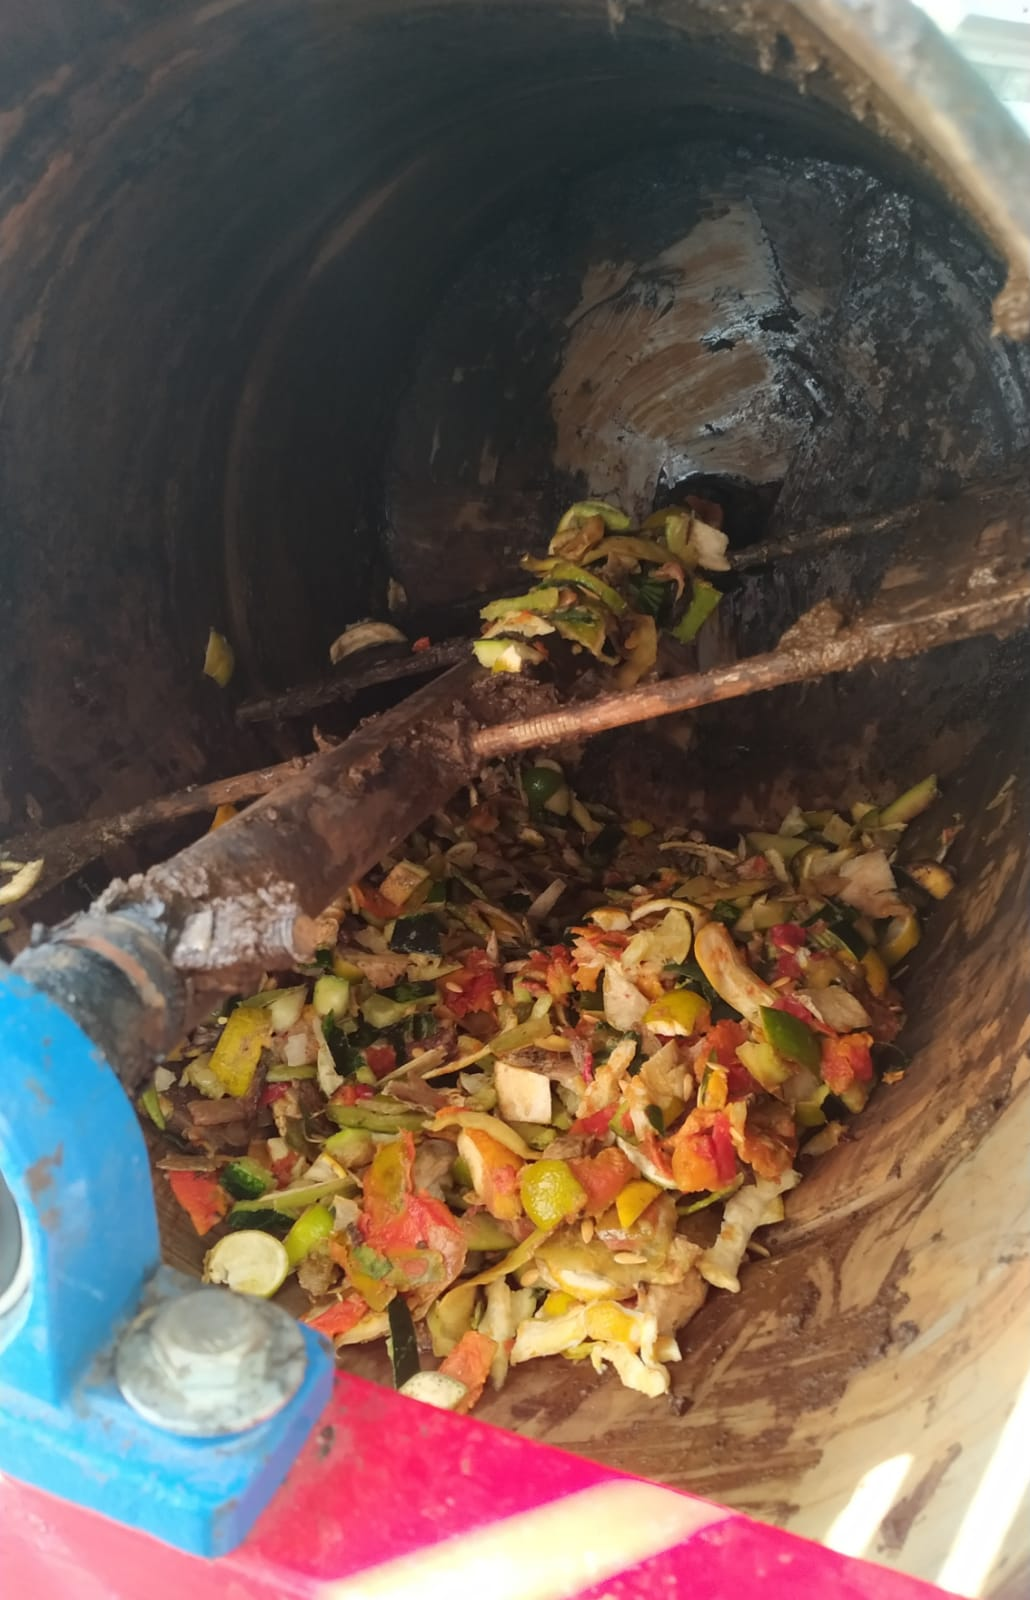
\includegraphics[scale=0.15]{images/Pruebas/Pruebas_compost/carga1.jpeg}
    \caption{Carga primera prueba}
    \label{fg:carga1}
\end{figure}
\clearpage

Esta prueba se realizó dentro del laboratorio de Trabajo Terminal 1, buscando completar un ciclo continuo de trabajo de 72 horas a lo largo de un fin de semana. Sin embargo, esta prueba se vio afectada por un corte de energía, el cual interrumpió el ciclo de trabajo después de un tiempo aproximado de 50 horas, cuando se encontraba en la segunda fase del crecimiento bacteriano.

Por lo que la materia que se logró obtener aún tenía algunos trozos reconocibles de verduras. A su vez, los desechos ya empezaban a adquirir un color marrón y se podían deshacer al contacto.

A pesar de tener un estado avanzado de descomposición, desprendían un olor agradable. También se encontraron con una humedad muy alta, siendo resultado de todos los líquidos lixiviados que se generaron durante el proceso y que quedaron atrapados en el contenedor.

\begin{figure}[h]
    \centering
    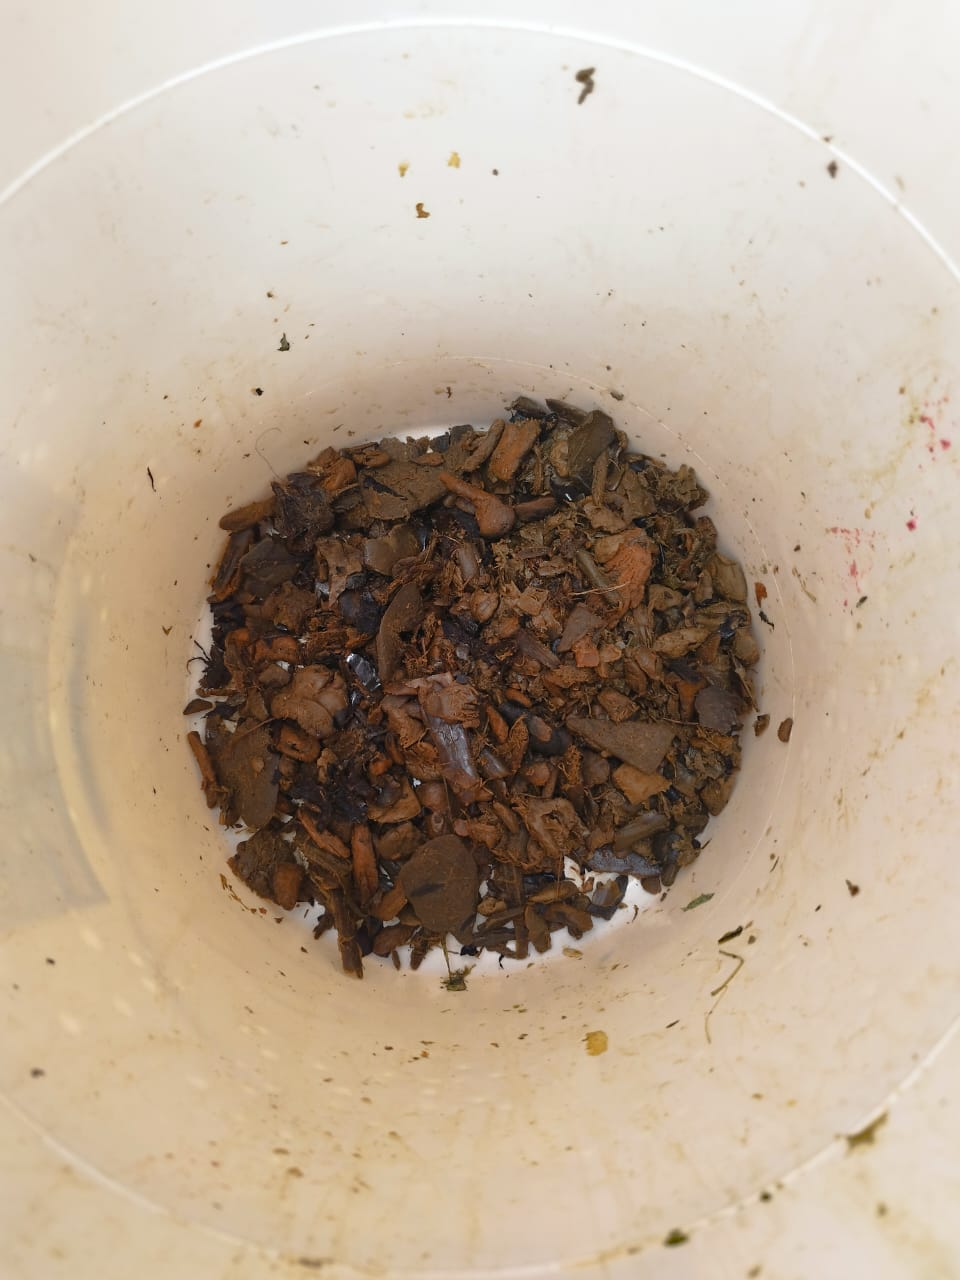
\includegraphics[scale=0.15]{images/Capitulo_Imple/S7/Val/Prueba1.jpeg}
    \caption{Primera muestra de composta obtenida}
    \label{fg:muestra1}
\end{figure}
\clearpage

\textbf{\textit{Segunda prueba}}

En esta segunda prueba se trabajó con 15 kg de residuos orgánicos, compuestos principalmente por desechos frutales, como melón, sandía y papaya, así como por residuos de verduras, entre los que se encontraban papa, jitomate y cebolla.

Para esta segunda prueba, se cambió el escenario de prueba, en donde se trasladó el dispositivo al anexo del laboratorio de Trabajo Terminal. Este espacio representa un área expuesta al aire libre, cubierta con láminas para evitar que se moje con la lluvia.

\begin{figure}[h]
    \centering
    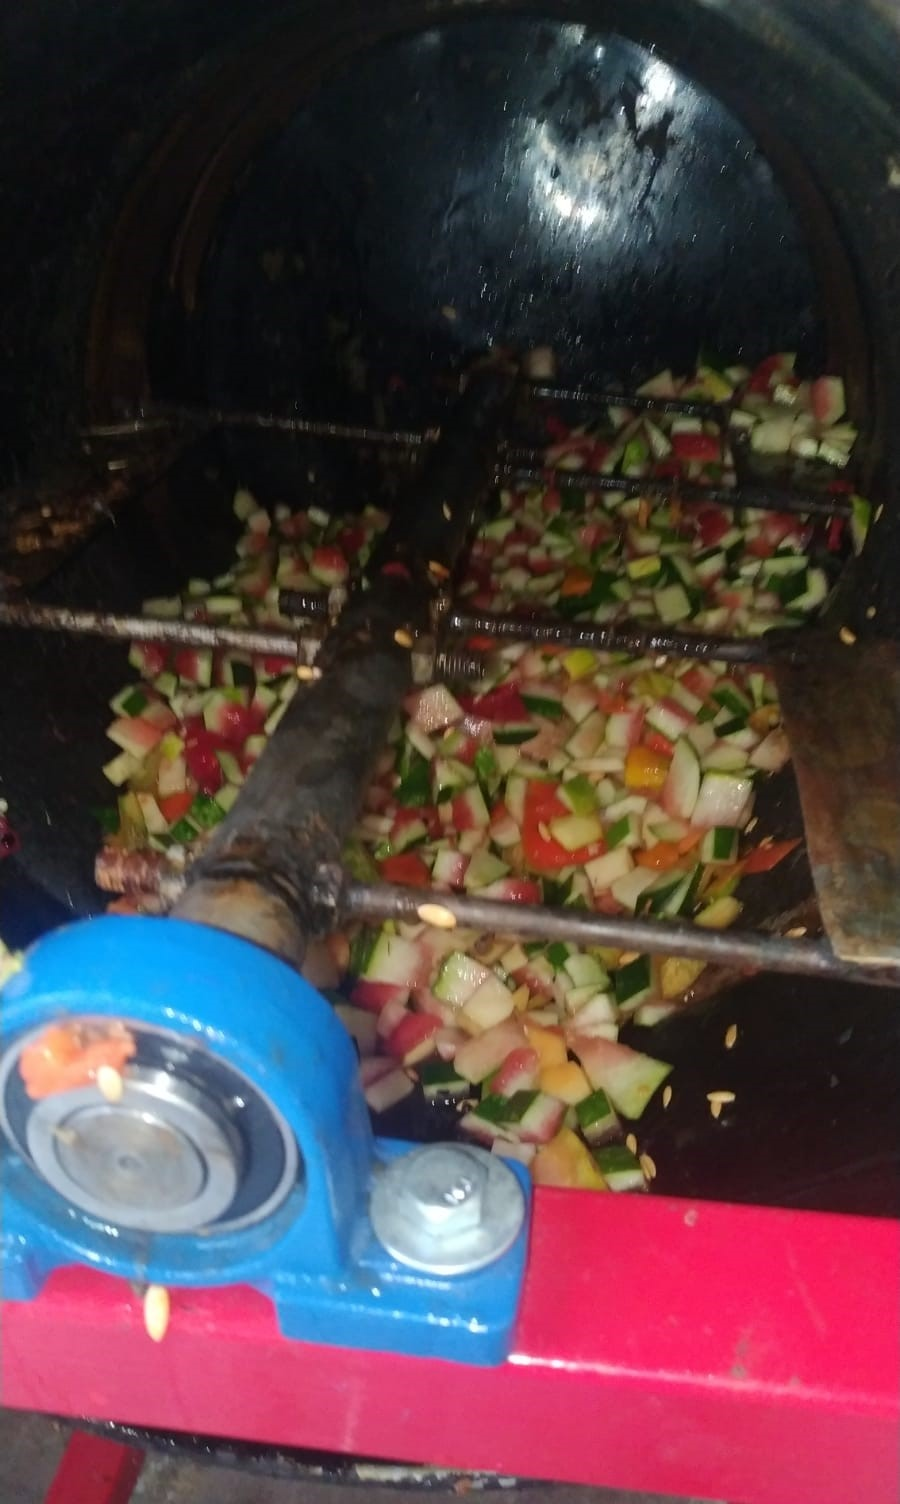
\includegraphics[scale=0.15]{images/Pruebas/Pruebas_compost/carga2.jpeg}
    \caption{Segunda carga}
    \label{fg:carga2}
\end{figure}
\clearpage

Esta prueba se hizo con una supervisión continua, ya que se realizó entre semana. Esta semana de pruebas contó con un clima muy frío que osciló entre los 8 °C y los 16 °C, por lo que se registraron mayores pérdidas de calor al interior del contenedor. De esta manera, el sistema para elevar la temperatura se mantuvo encendido más tiempo y representó un mayor consumo de energía.

A pesar de esto, se logró mantener un ciclo completo de 72 horas, por lo que, al final, fue posible obtener una mezcla más homogénea, con un peso de 6.4 kg. Esta materia ya contaba con un color marrón más intenso y un olor agradable, como a ponche de frutas. De igual manera, presentaba una consistencia bastante húmeda; por tal motivo, se procedió a realizar otro ciclo de 24 horas con el fin de eliminar el exceso de agua. Sin embargo, el resultado no distaba de la muestra obtenida previamente, ya que la mezcla seguía presentando una cantidad considerable de agua.

\begin{figure}[h]
    \centering
    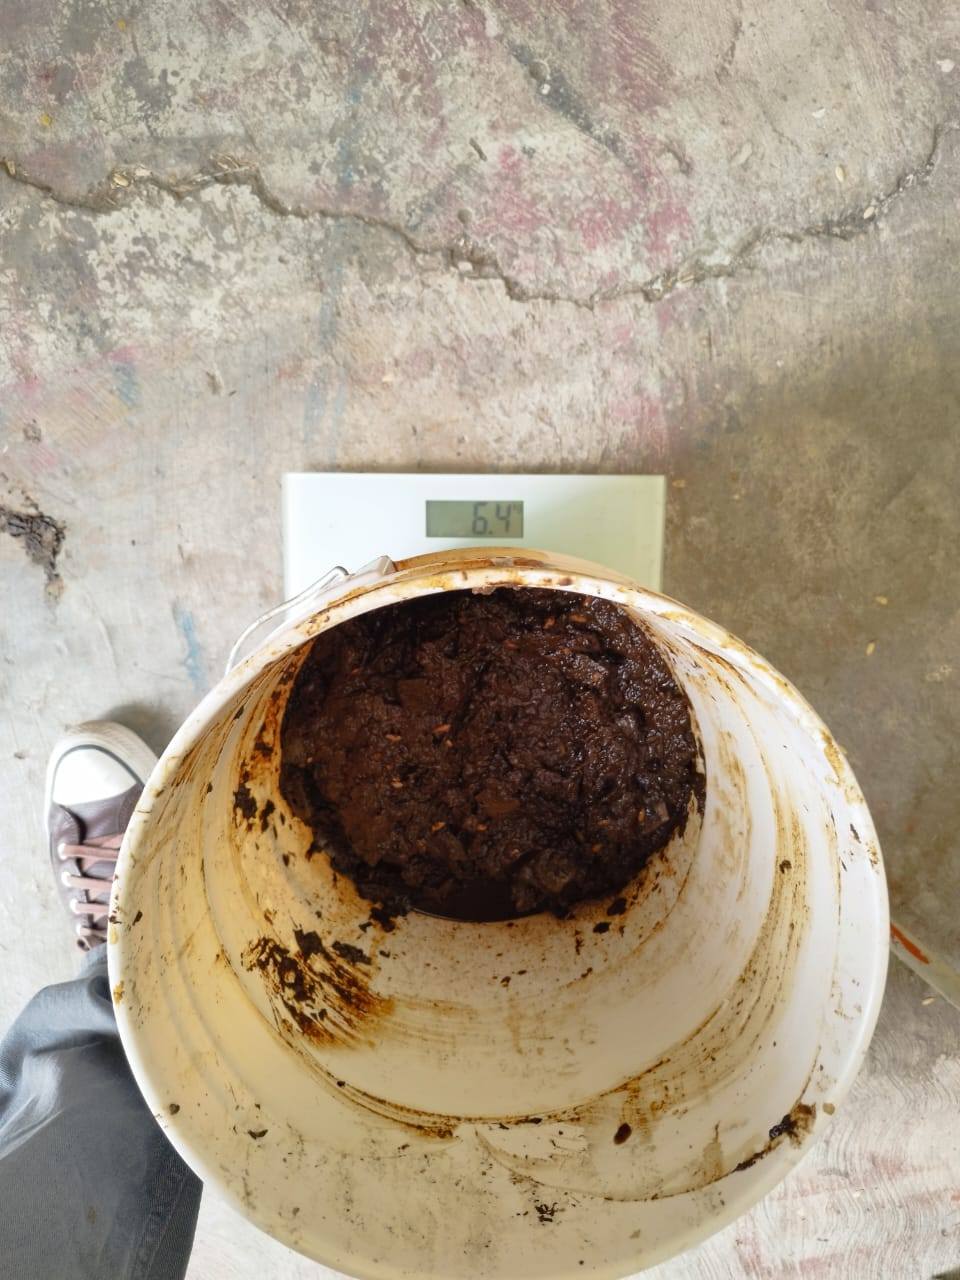
\includegraphics[scale=0.15]{images/Capitulo_Imple/S7/Val/Prueba2.jpeg}
    \caption{Segunda muestra de composta obtenida}
    \label{fg:muestra2}
\end{figure}
\clearpage

\textbf{\textit{Tercera prueba}}

Para la tercera prueba se emplearon cerca de 13.8 kg de residuos. De igual manera que en los procesos anteriores, se utilizaron desechos frutales, como melón, sandía y papaya, y también se emplearon desechos provenientes de verduras, como papa, jitomate y zanahoria.

Sin embargo, en esta prueba se trituró la totalidad de los desechos, obteniendo partículas de aproximadamente 3 mm de tamaño. Como se puede observar en la siguiente imagen, la mezcla presenta una apariencia más homogénea, debido a que los residuos triturados adquieren prácticamente una misma tonalidad naranja. Por otro lado, es importante mencionar que las frutas y verduras utilizadas en esta prueba presentaban una apariencia seca antes de la trituración, por lo que se observó una menor cantidad de líquidos durante este proceso.

\begin{figure}[h]
    \centering
    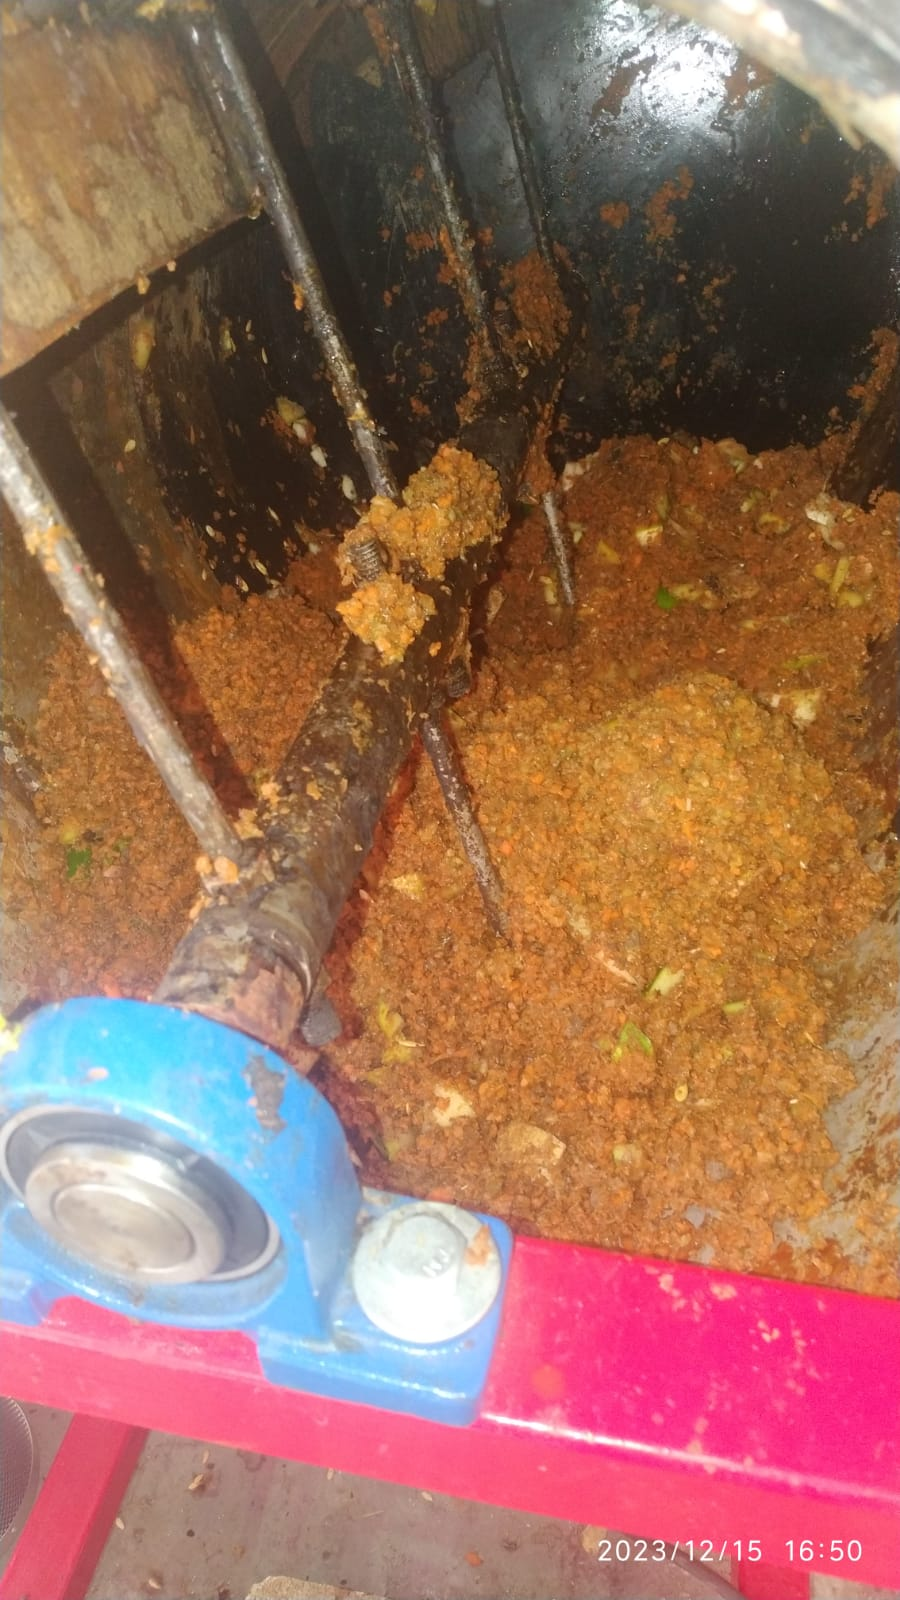
\includegraphics[scale=0.15]{images/Pruebas/Pruebas_compost/carga3.jpeg}
    \caption{Tercera prueba carga}
    \label{fg:carga3}
\end{figure}

Esta prueba duró 72 horas, obteniéndose 5.6 kg. Como se puede observar en la siguiente imagen, presenta una apariencia más cercana a la tierra empleada para las macetas, pues la partícula es más fina y presenta un color café obscuro además de un olor agradable, como a durazno. Otra característica a notar es que la cantidad de agua es mínima. Además, al apretar la mezcla con la mano y soltarla, esta se deshace como si se tratara de tierra. Los elementos de mayor tamaño fueron cáscaras que no pasaron por el triturador.

\begin{figure}[h]
    \centering
    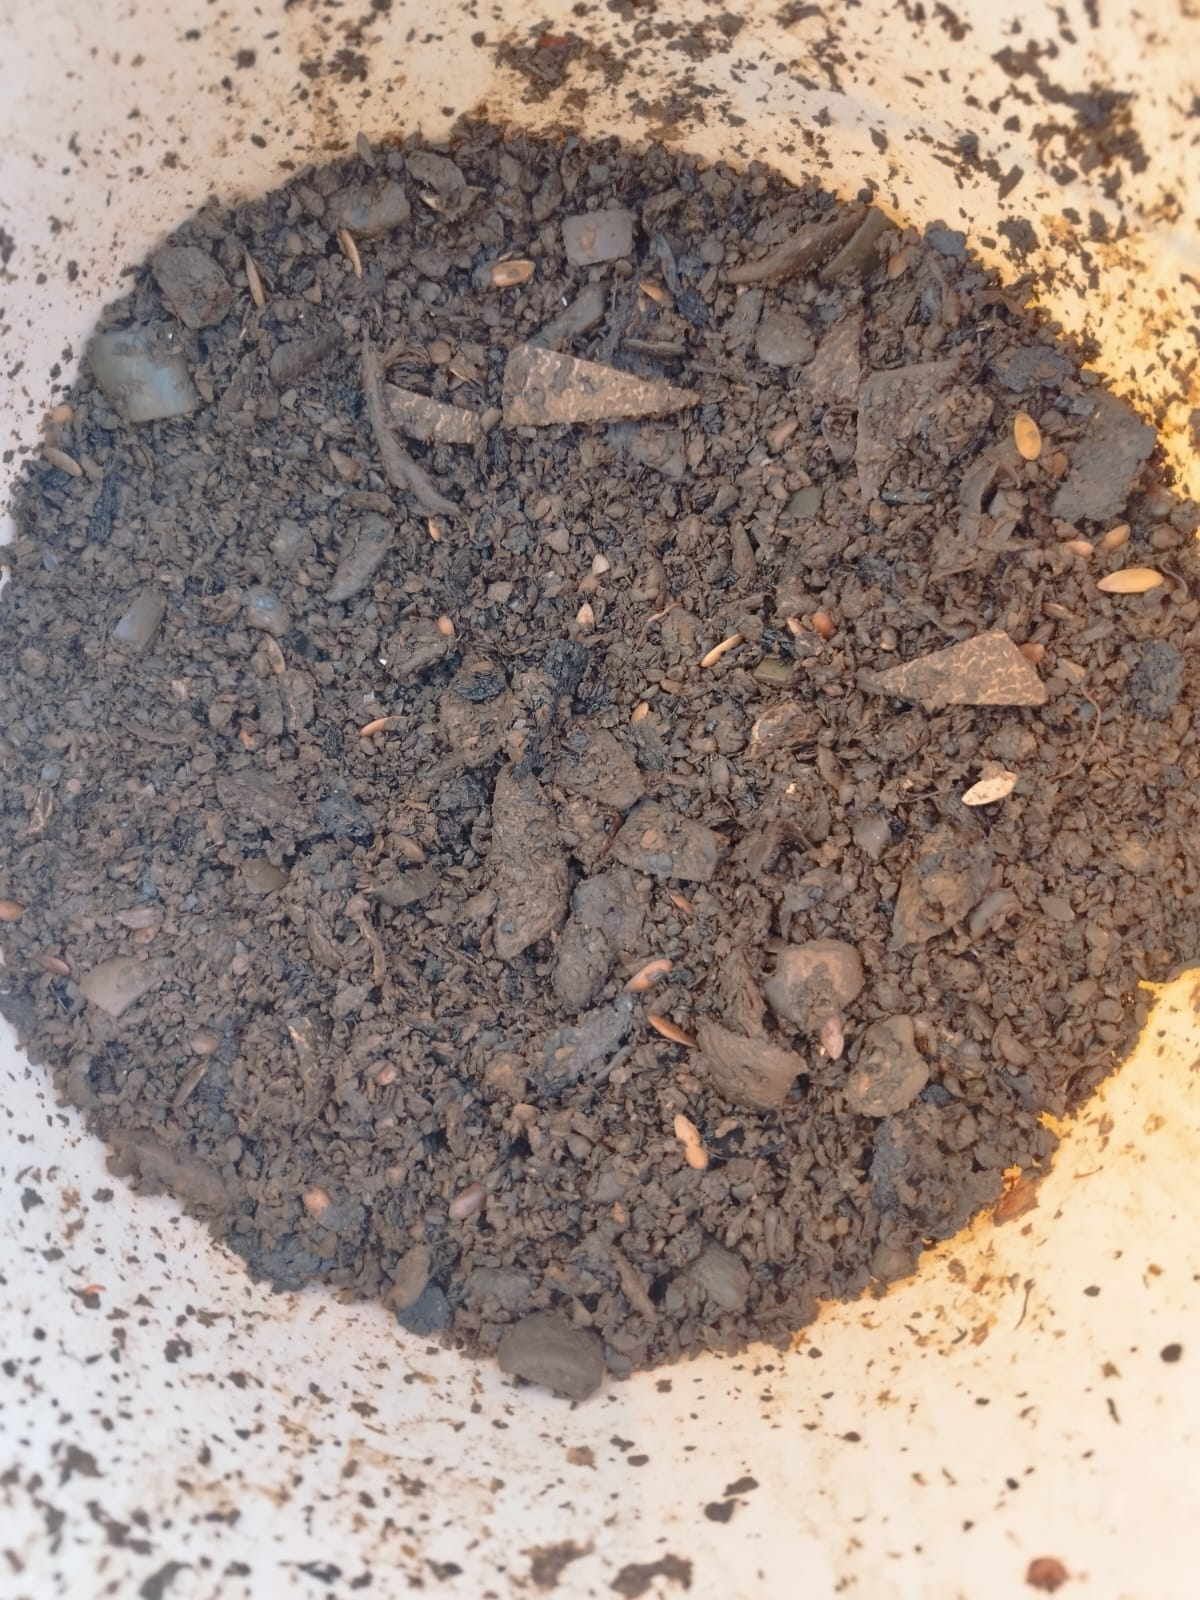
\includegraphics[scale=0.15]{images/Pruebas/Pruebas_compost/descarga3.jpeg}
    \caption{Tercera prueba descarga}
    \label{fg:descarga3}
\end{figure}

\textbf{\textit{Cuarta prueba}}

En esta prueba se introdujeron aproximadamente 14.1 kg de desechos, compuestos por frutas como sandía, melón y papaya, así como por verduras, entre las que se encontraban zanahoria y papa. Del total de los residuos, la mitad fue triturada, mientras que la otra mitad se introdujo únicamente picada. El proceso se mantuvo durante un ciclo de 72 horas, al término del cual se obtuvieron 6.1 kg de compost. Como se puede observar en la siguiente imagen, la mezcla presenta una apariencia homogénea y un nivel de humedad moderado. Asimismo, se percibe un olor agradable con características frutales.

\begin{figure}[h]
    \centering
    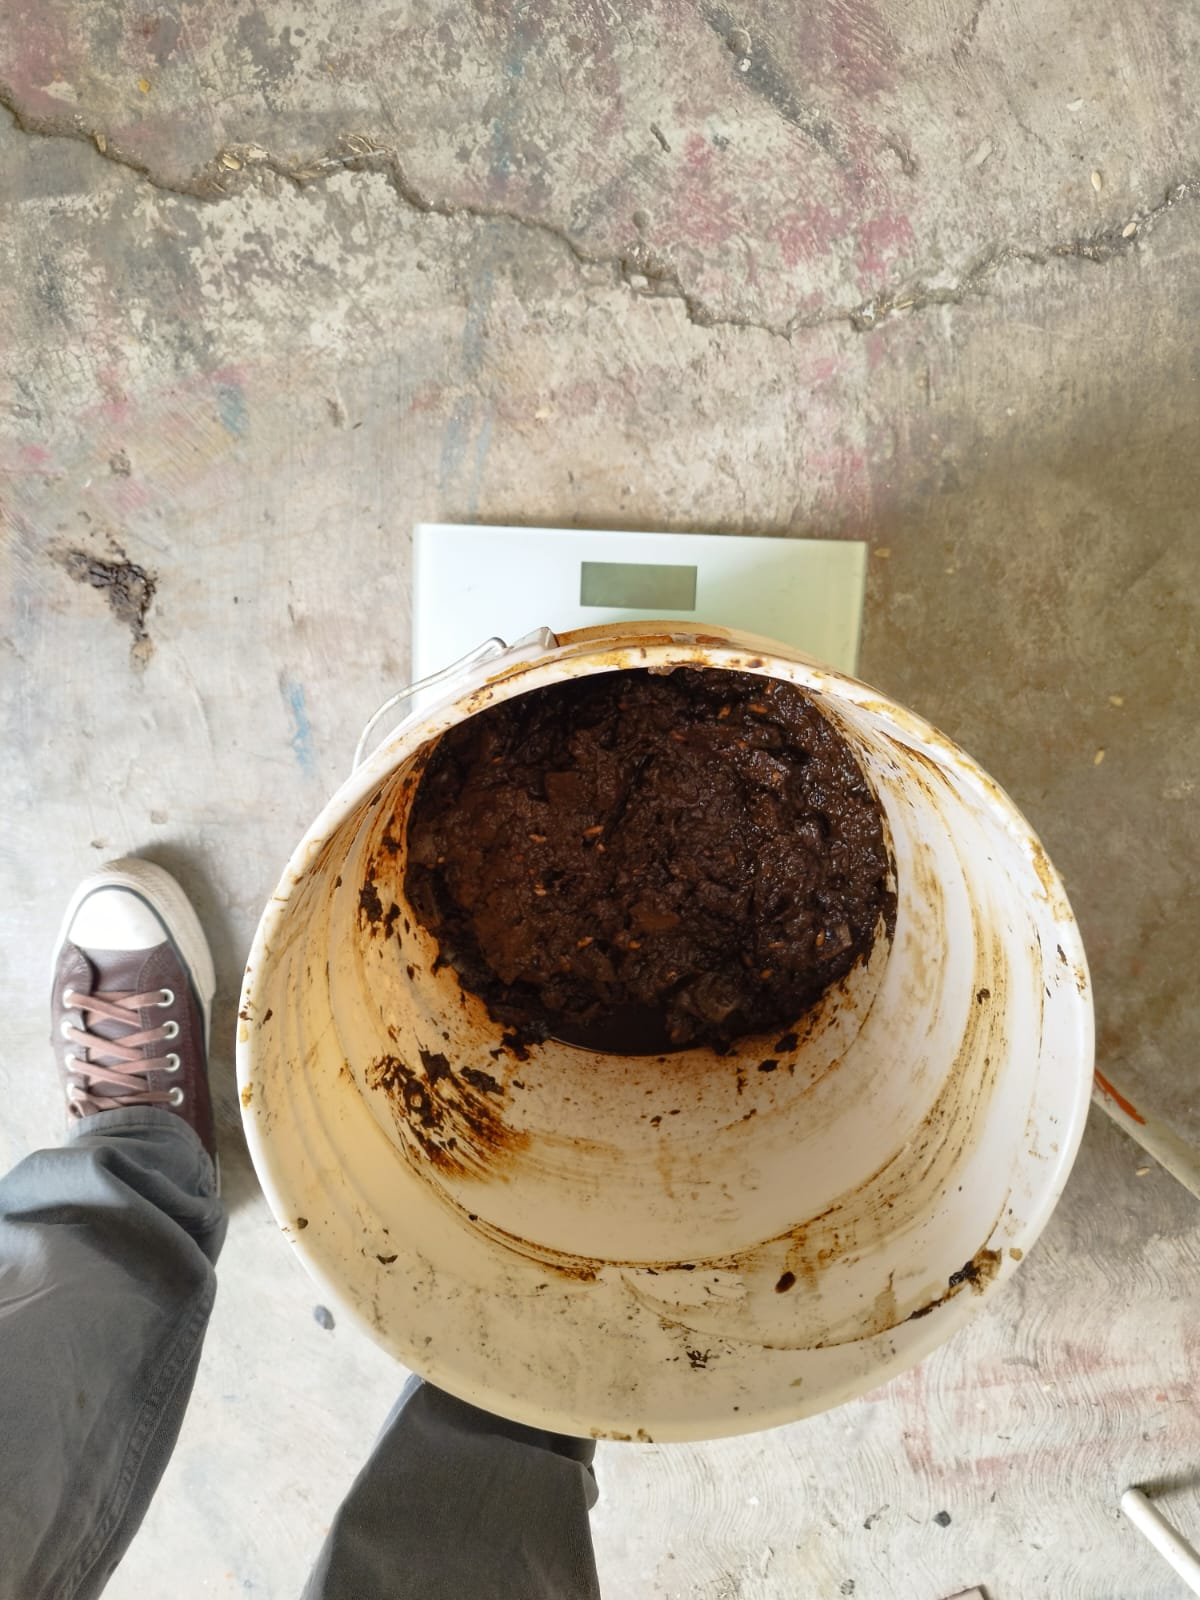
\includegraphics[scale=0.15]{images/Pruebas/Pruebas_compost/descarga4.jpeg}
    \caption{Cuarta prueba descarga}
    \label{fg:descarga4}
\end{figure}

\textbf{\textit{Quinta prueba}}

Cabe destacar, que en esta prueba se introdujo la mayor cantidad de desechos registrada para este proyecto, teniendo un total de 15.5 Kg de frutas y verduras. Para esta ocasión no se trituró la mezcla, sino que solamente se picó y se colocó en el contenedor.

\begin{figure}[h]
    \centering
    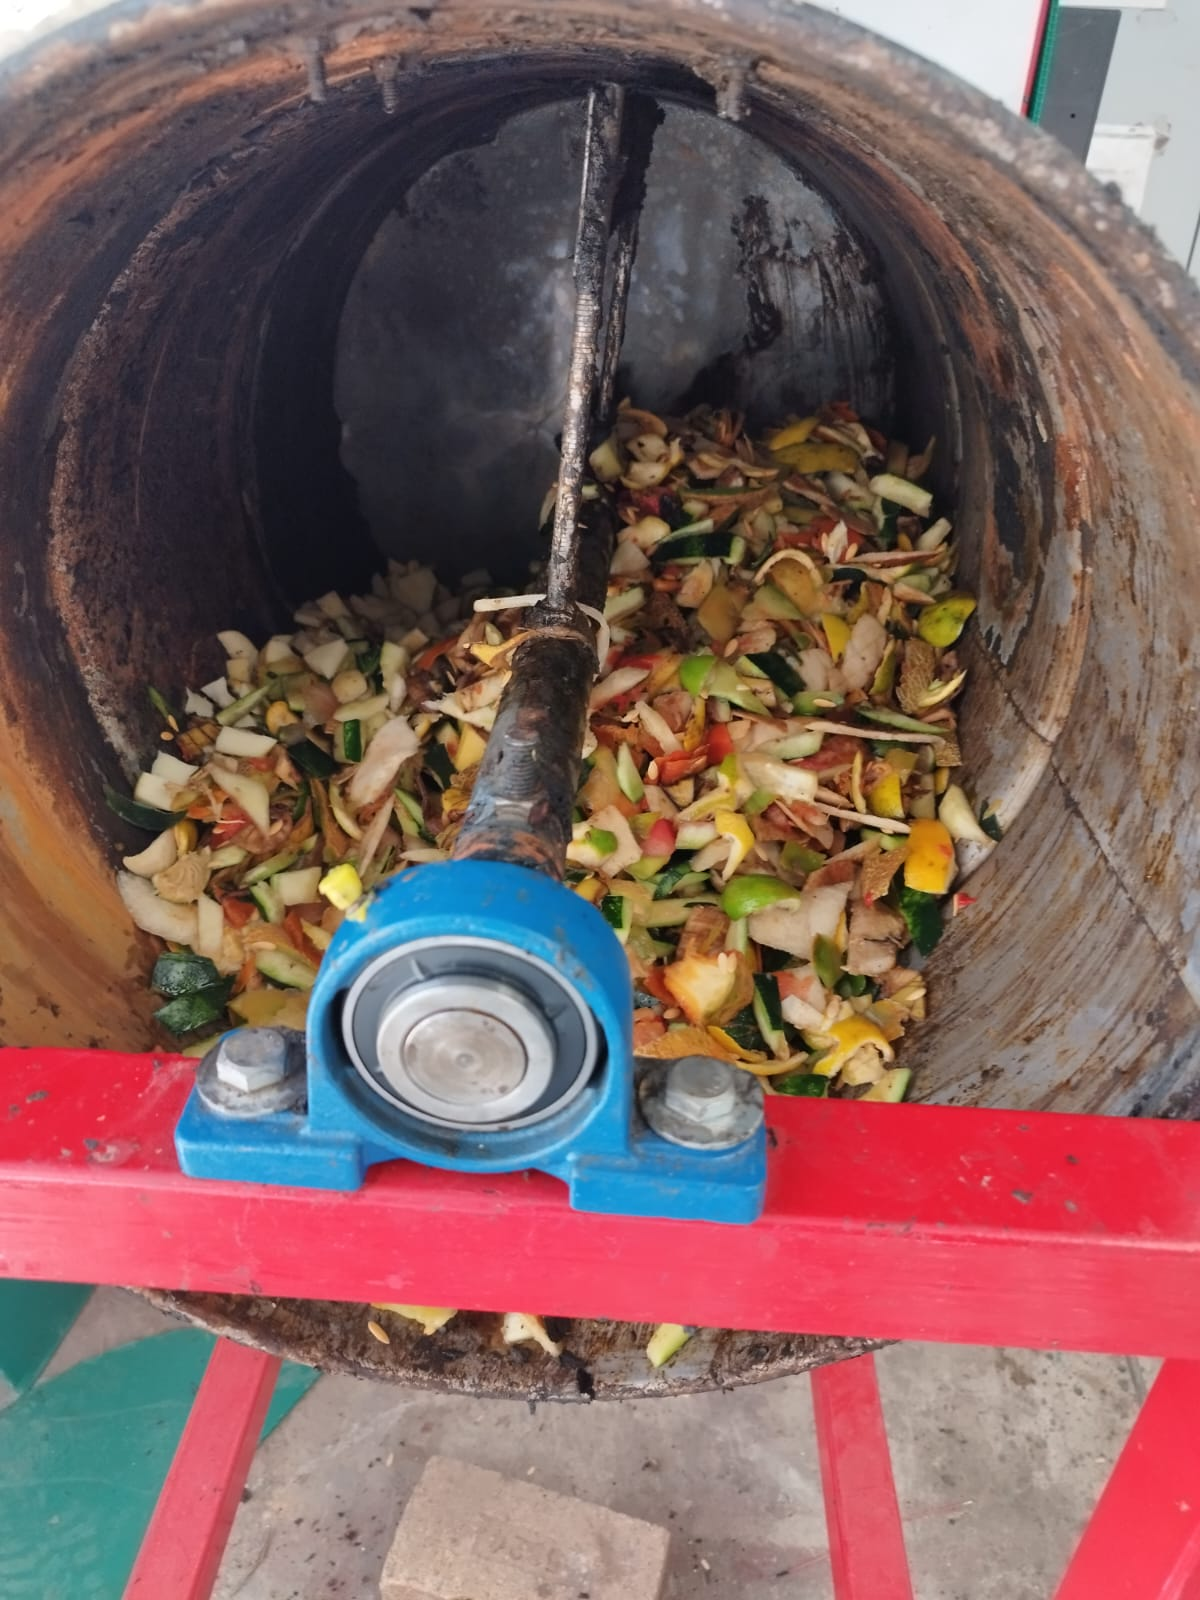
\includegraphics[scale=0.15]{images/Pruebas/Pruebas_compost/carga5.jpeg}
    \caption{Quinta prueba carga}
    \label{fg:carga5}
\end{figure}

Es importante señalar que la fruta y verdura eran frescas, conteniendo una gran cantidad de agua. Se hace hincapié en este detalle, pues a lo largo de estas pruebas se ha observado que el estado en el que ingresan los desechos influye en el resultado final. Como se puede observar en la siguiente imagen, la mezcla presenta una consistencia parecida al mole o al lodo, lo que indicaría que aún presenta un porcentaje de agua considerable. Por otro lado, se continúa obteniendo una mezcla homogénea de color café oscuro y de olor agradable. Al final de este intento se extrajeron 7.5 kg de compost.

\begin{figure}[h]
    \centering
    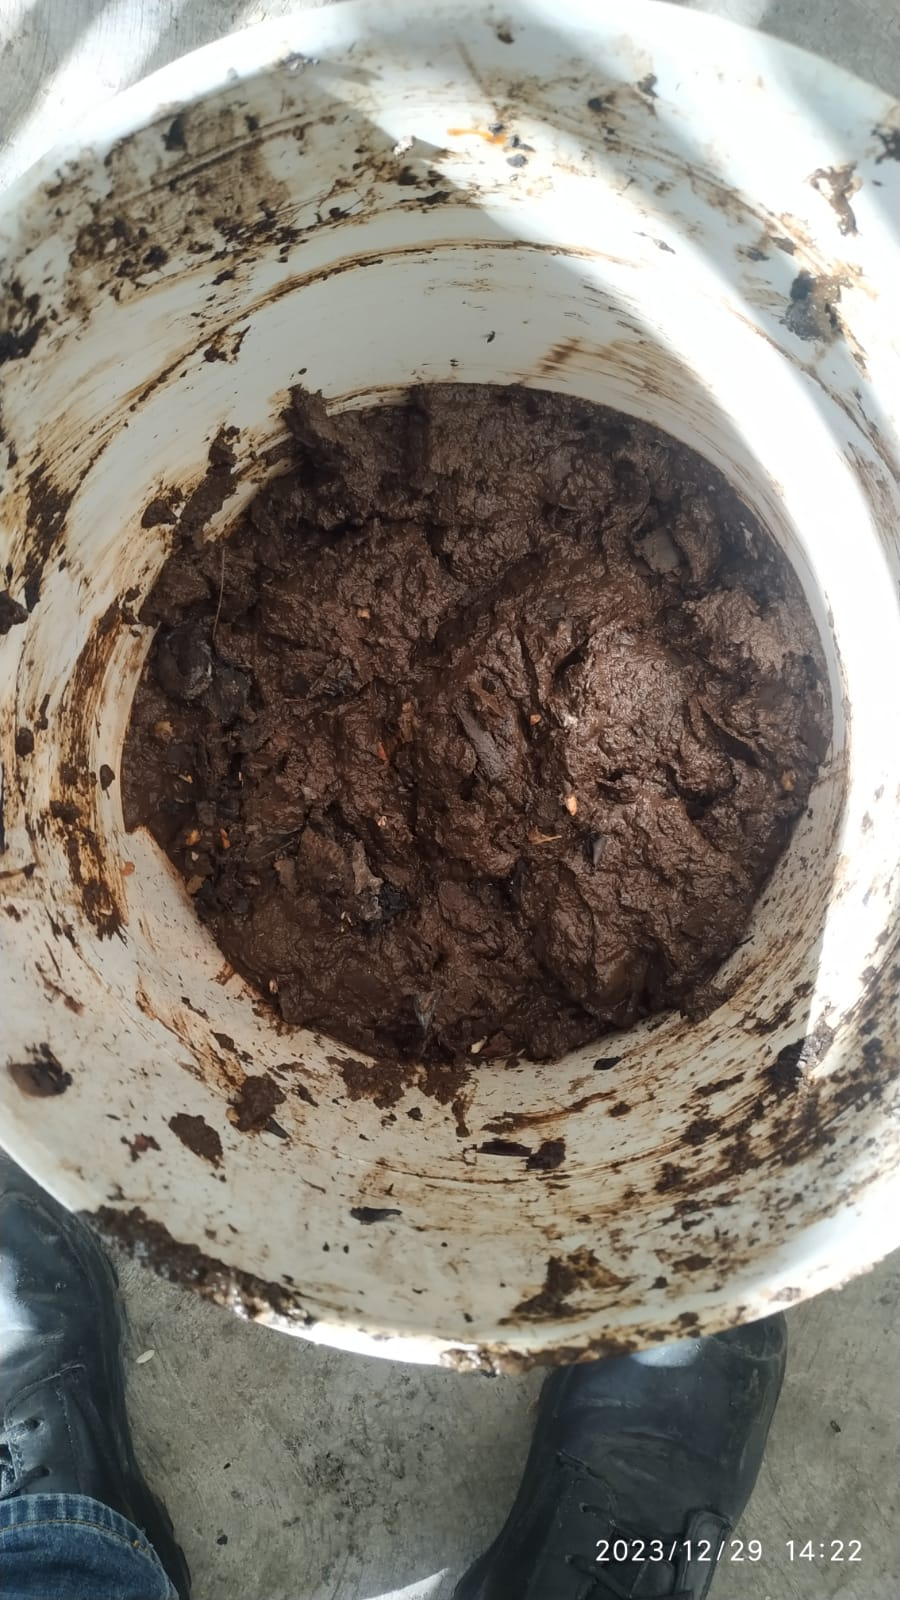
\includegraphics[scale=0.15]{images/Pruebas/Pruebas_compost/descarga5.jpeg}
    \caption{Quinta prueba descarga}
    \label{fg:descarga5}
\end{figure}

\textbf{\textit{Sexta prueba}}

Para la última prueba se introdujeron 7.2 kg de desperdicios entre fruta y verdura siendo de las pruebas con menor carga registrada.

\begin{figure}[h]
    \centering
    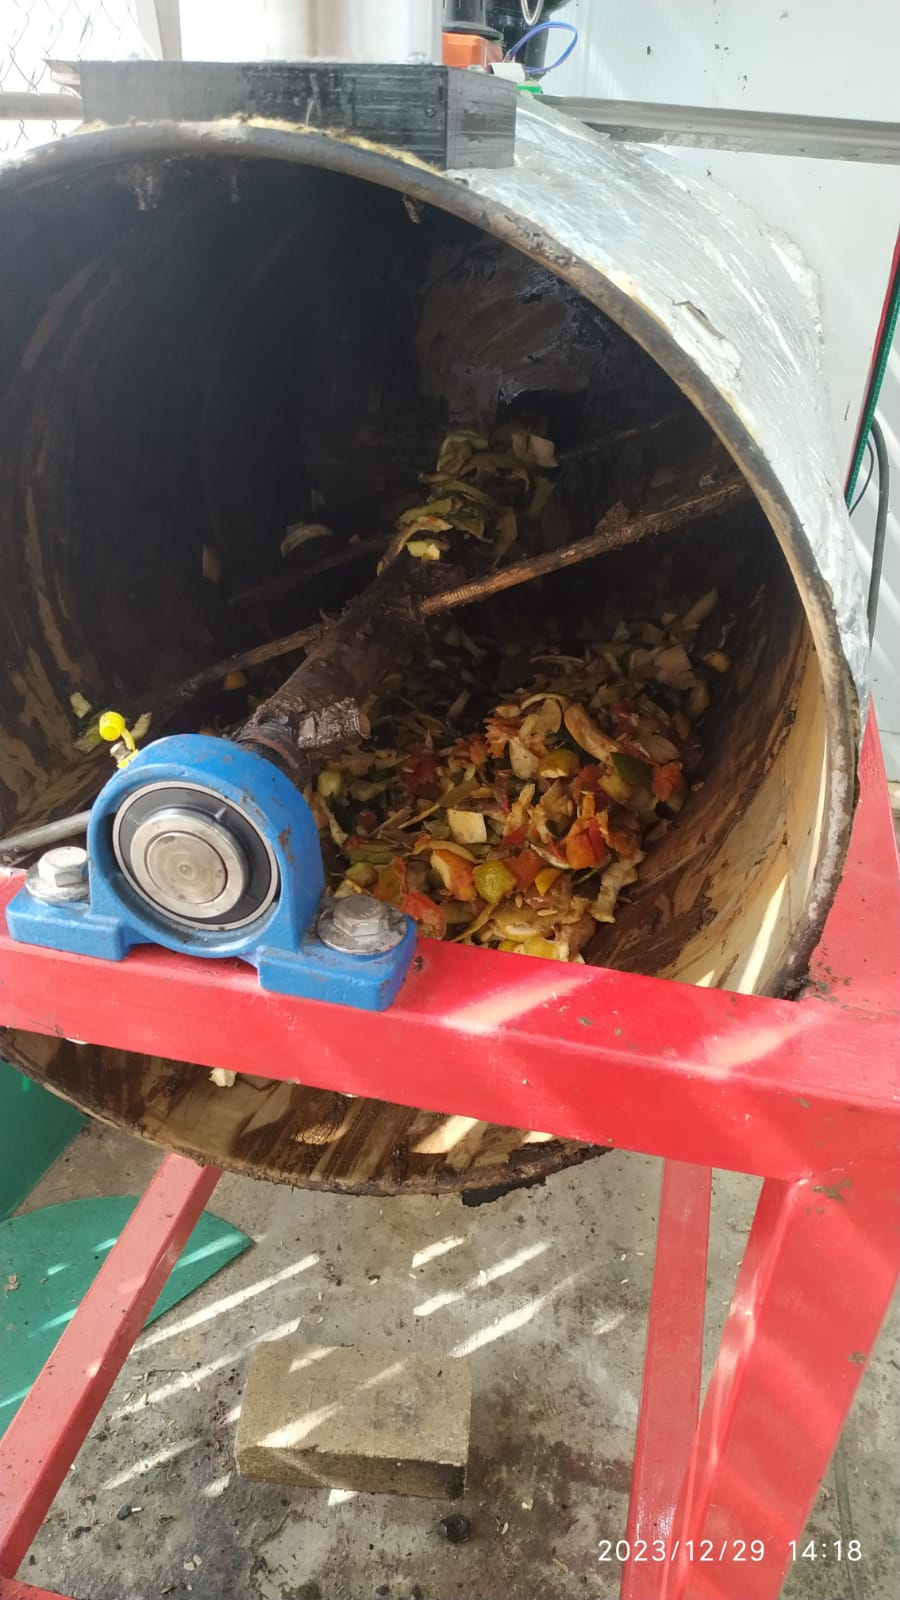
\includegraphics[scale=0.15]{images/Pruebas/Pruebas_compost/carga6.jpeg}
    \caption{Sexta prueba carga}
    \label{fg:carga6}
\end{figure}

Desafortunadamente en el lugar que se encuentra el dispositivo estuvo presentando cortes de energía eléctrica, se estima que el ciclo se detuvo a las 40 horas del proceso obteniéndose el siguiente resultado:

\begin{figure}[h]
    \centering
    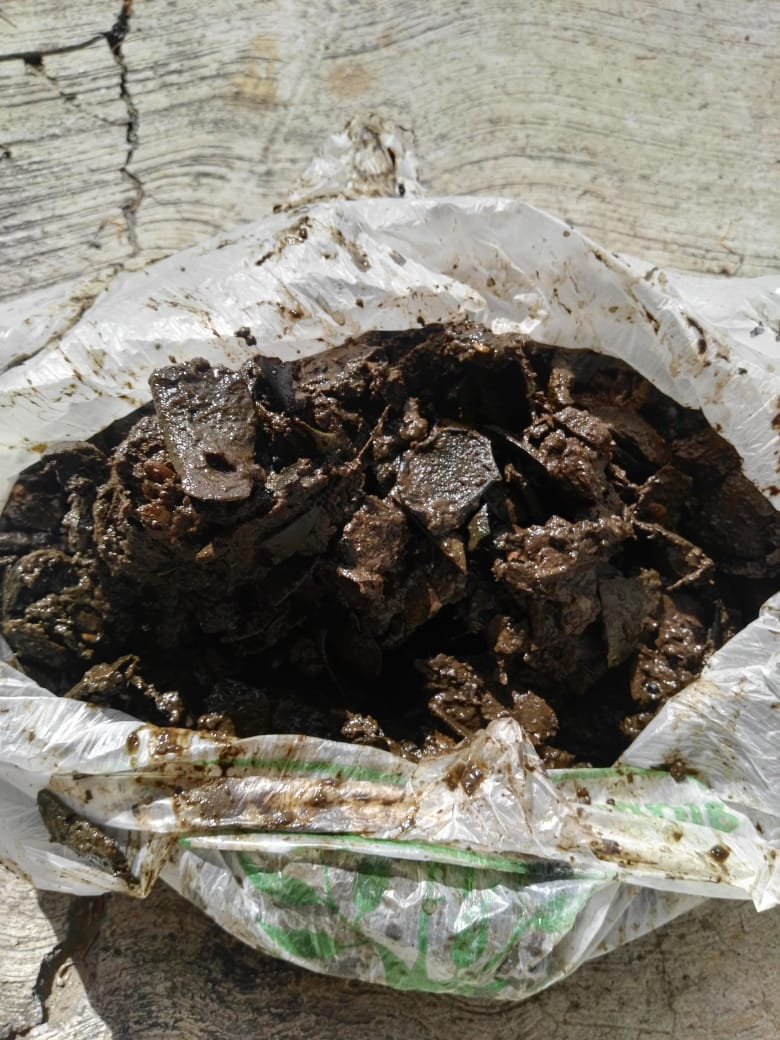
\includegraphics[scale=0.15]{images/Pruebas/Pruebas_compost/descarga6.jpeg}
    \caption{Sexta prueba descarga}
    \label{fg:descarga6}
\end{figure}

Como se puede observar, se trata de una mezcla heterogénea en donde claramente se distingue la mayoría de los residuos, añadiendo que la cantidad de agua contenida resulta exagerada. Esto, a consecuencia de la interrupción del proceso, presenta un olor desagradable, similar al de un alimento en descomposición, debido también al tiempo que pasó dentro del contenedor. Y, aunque este intento se considera fallido, se ha decidido registrarlo, puesto que brinda cierta retroalimentación sobre posibles mejoras a futuro. Por otro lado, es importante señalar que las muestras exitosas fueron consistentes, ya que la cantidad de compost obtenida es cerca del 43\% del total ingresado.

\clearpage

\textbf{\textit{Pruebas de pH}}

Para verificar la calidad del compost obtenido, se realizaron pruebas de pH para verificar la estabilidad de la mezcla. Se muestran las imágenes de las pruebas realizadas y los resultados obtenidos en la Tabla \ref{tab:pruebas_compostaje}. Es importante señalar que, aunque se llevaron a cabo seis pruebas de compostaje, solo se realizaron mediciones de pH y registro fotográfico para las primeras cinco muestras. La sexta prueba fue interrumpida y no cuenta con imágenes ni medición de pH, por lo que se incluye únicamente en la tabla resumen como caso fallido.

El proceso completo de medición se documenta en las Figuras \ref{fg:muestra1_proceso} a \ref{fg:muestra5_proceso}, donde cada figura ilustra tres etapas clave: el pesaje de la muestra, la comparativa colorimétrica y la lectura con el pHmetro. Estas imágenes permiten corroborar visualmente las condiciones de cada muestra y respaldan los resultados numéricos presentados en la Tabla \ref{tab:pruebas_compostaje}.

La primera muestra, correspondiente a la prueba 1, se caracterizó por una mezcla homogénea de color marrón intenso y un olor afrutado, similar al ponche de frutas. Sin embargo, presentó un contenido de humedad excesivo que no pudo corregirse ni siquiera tras 24 horas adicionales de ciclo, lo que se refleja en un pH final de 8.83.

\begin{figure}[htbp]
    \centering
    \begin{subfigure}[b]{0.28\textwidth}
        \centering
        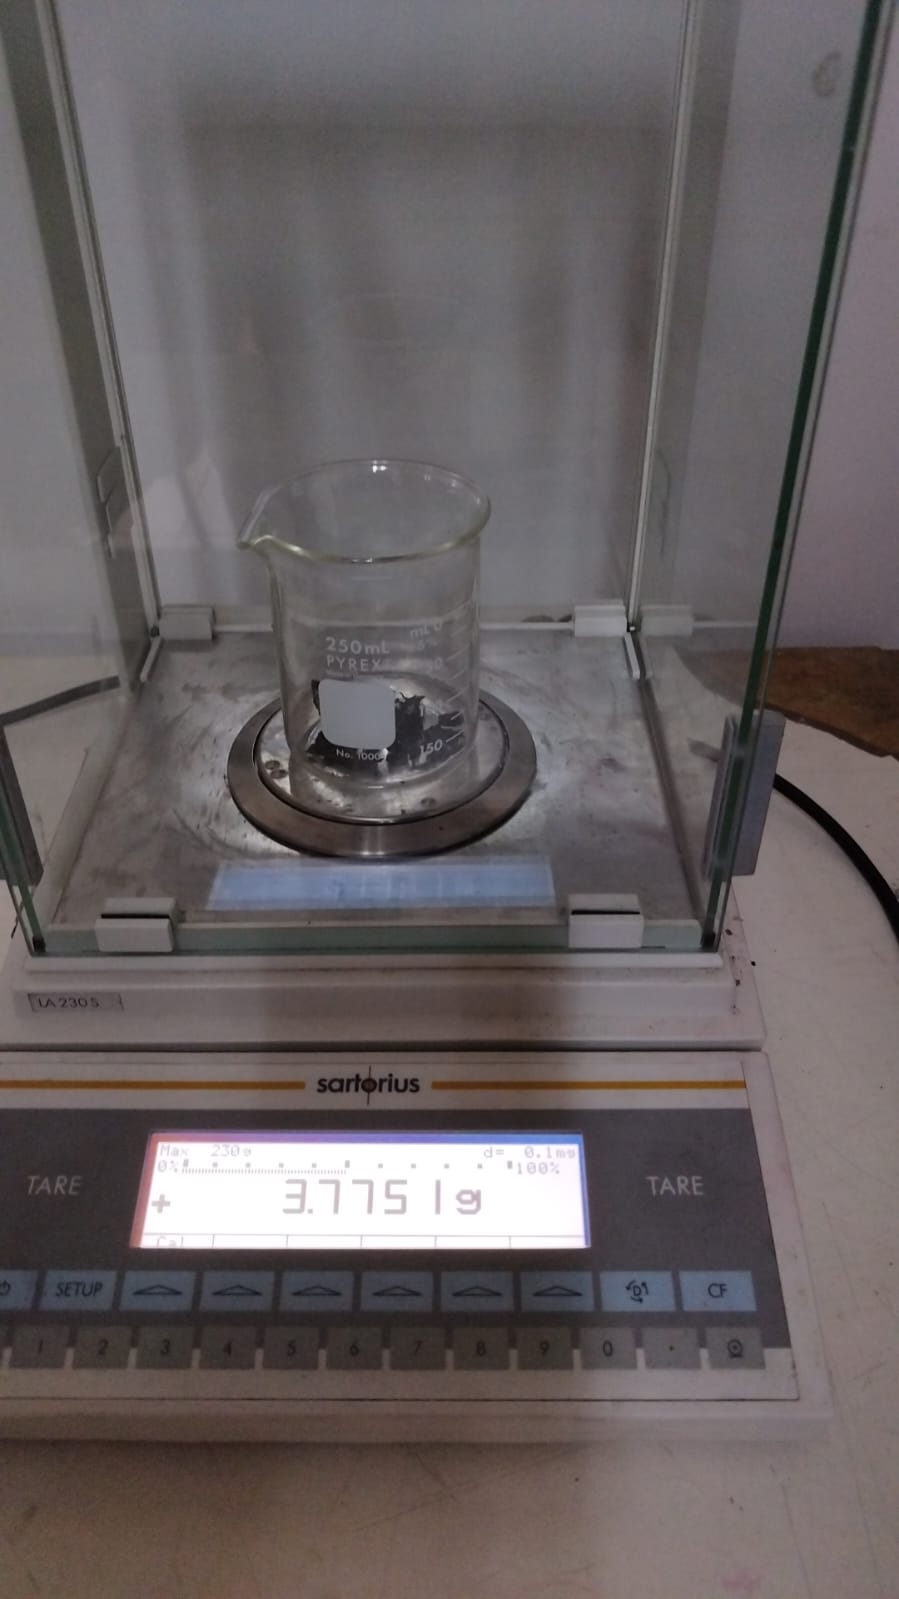
\includegraphics[width=\textwidth]{images/Pruebas/Resultados/muestra_1.jpeg}
        \caption{Pesaje}
        \label{fg:m1_pesaje}
    \end{subfigure}
    \hfill
    \begin{subfigure}[b]{0.32\textwidth}
        \centering
        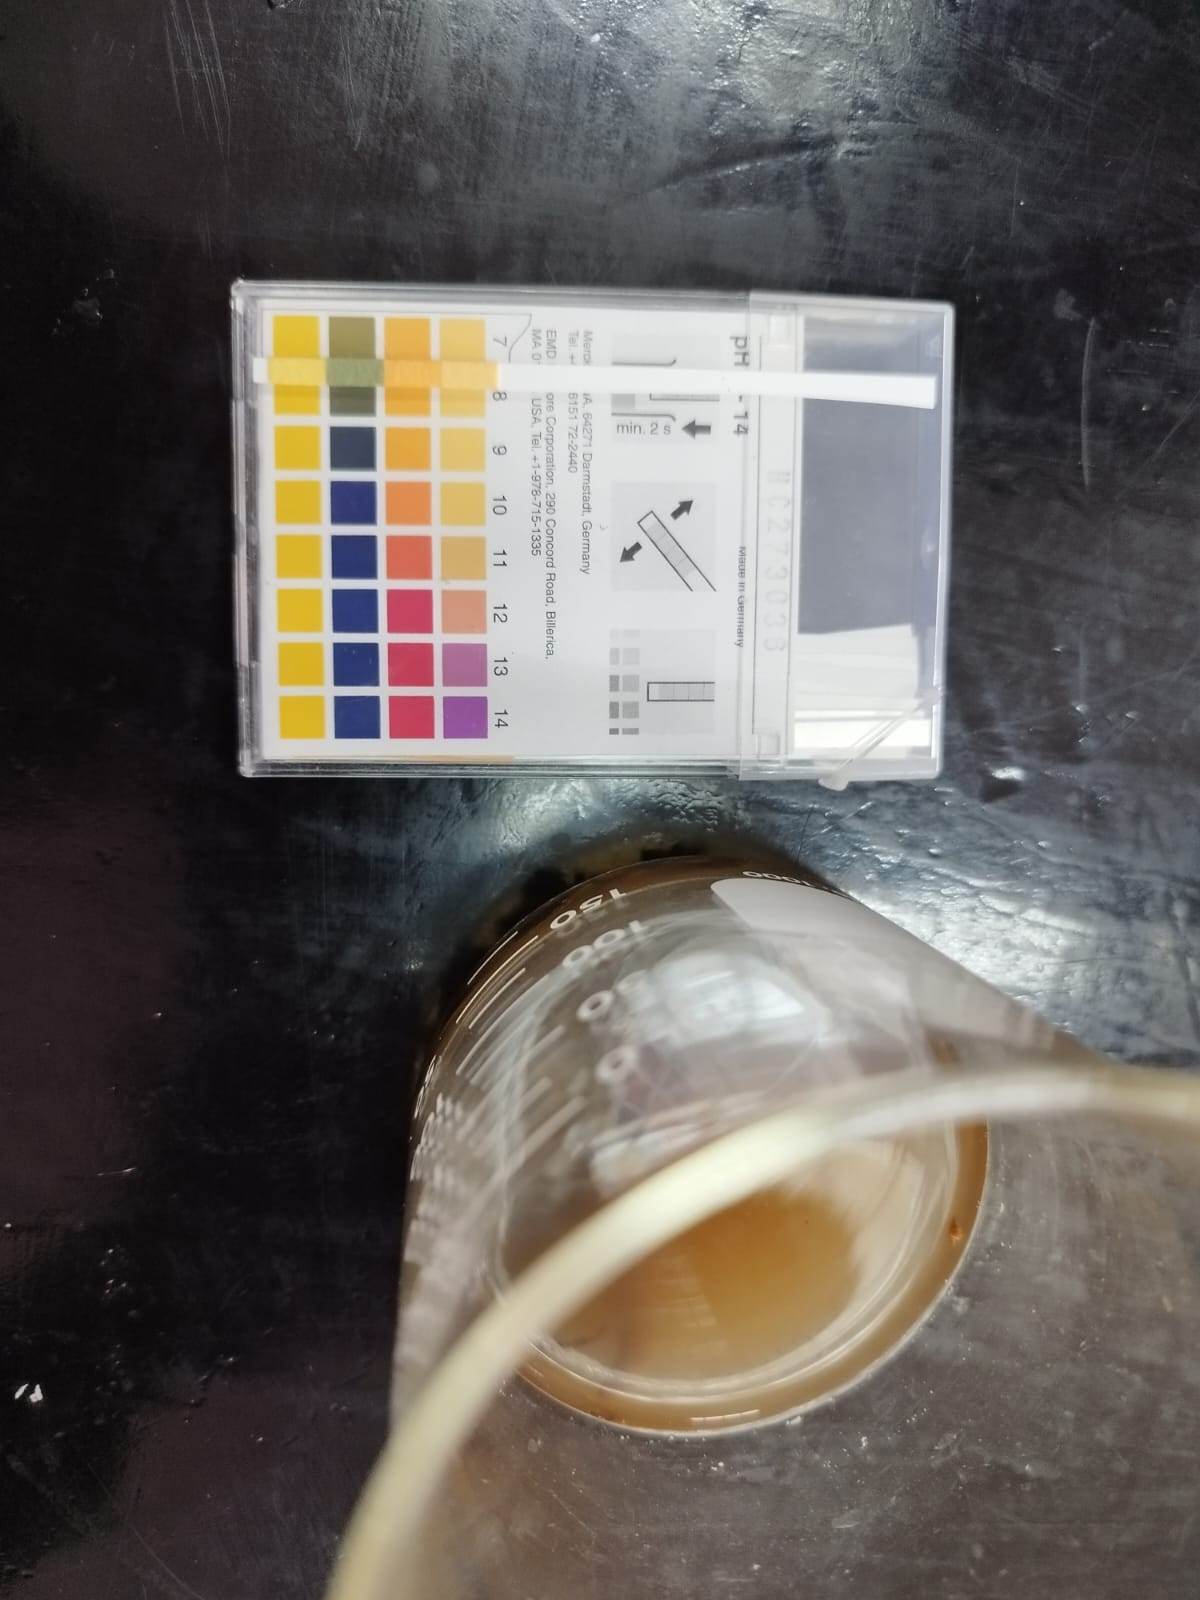
\includegraphics[width=\textwidth]{images/Pruebas/Resultados/muestra_1_colorimetria.jpeg}
        \caption{Comparativa colorimétrica}
        \label{fg:m1_color}
    \end{subfigure}
    \hfill
    \begin{subfigure}[b]{0.32\textwidth}
        \centering
        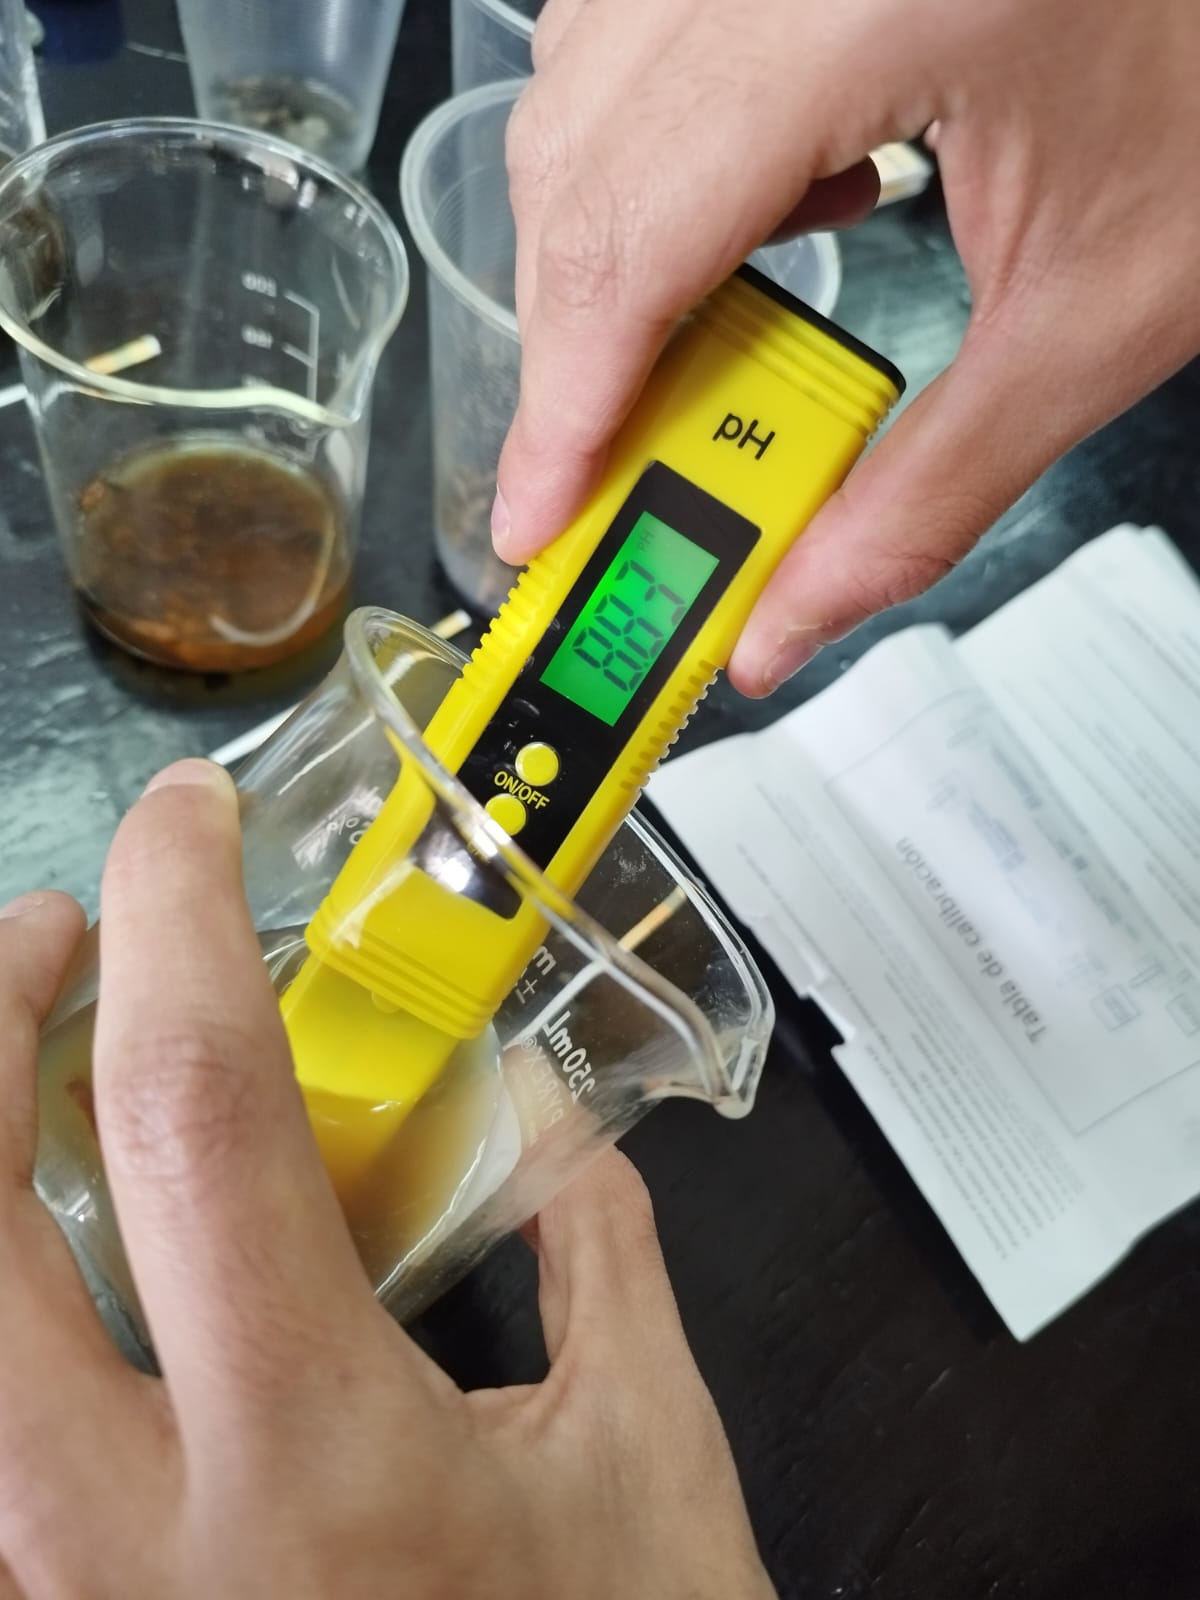
\includegraphics[width=\textwidth]{images/Pruebas/Resultados/muestra_1_phmetro.jpeg}
        \caption{Lectura de pHmetro}
        \label{fg:m1_ph}
    \end{subfigure}
    \caption{Proceso de medición de pH — Muestra 1}
    \label{fg:muestra1_proceso}
\end{figure}

En Figura \ref{fg:muestra1_proceso} se presenta la muestra durante las etapas de pesaje, comparación colorimétrica y medición con el pHmetro. 

La segunda muestra, asociada a la prueba 2, mantuvo la misma problemática de humedad excesiva que la primera, sin que se lograra reducir el agua durante el proceso. Aunque no se reportó la cantidad de compost obtenido, el pH final fue de 7.96, ligeramente superior al de la muestra anterior.

\begin{figure}[htbp]
    \centering
    \begin{subfigure}[b]{0.28\textwidth}
        \centering
        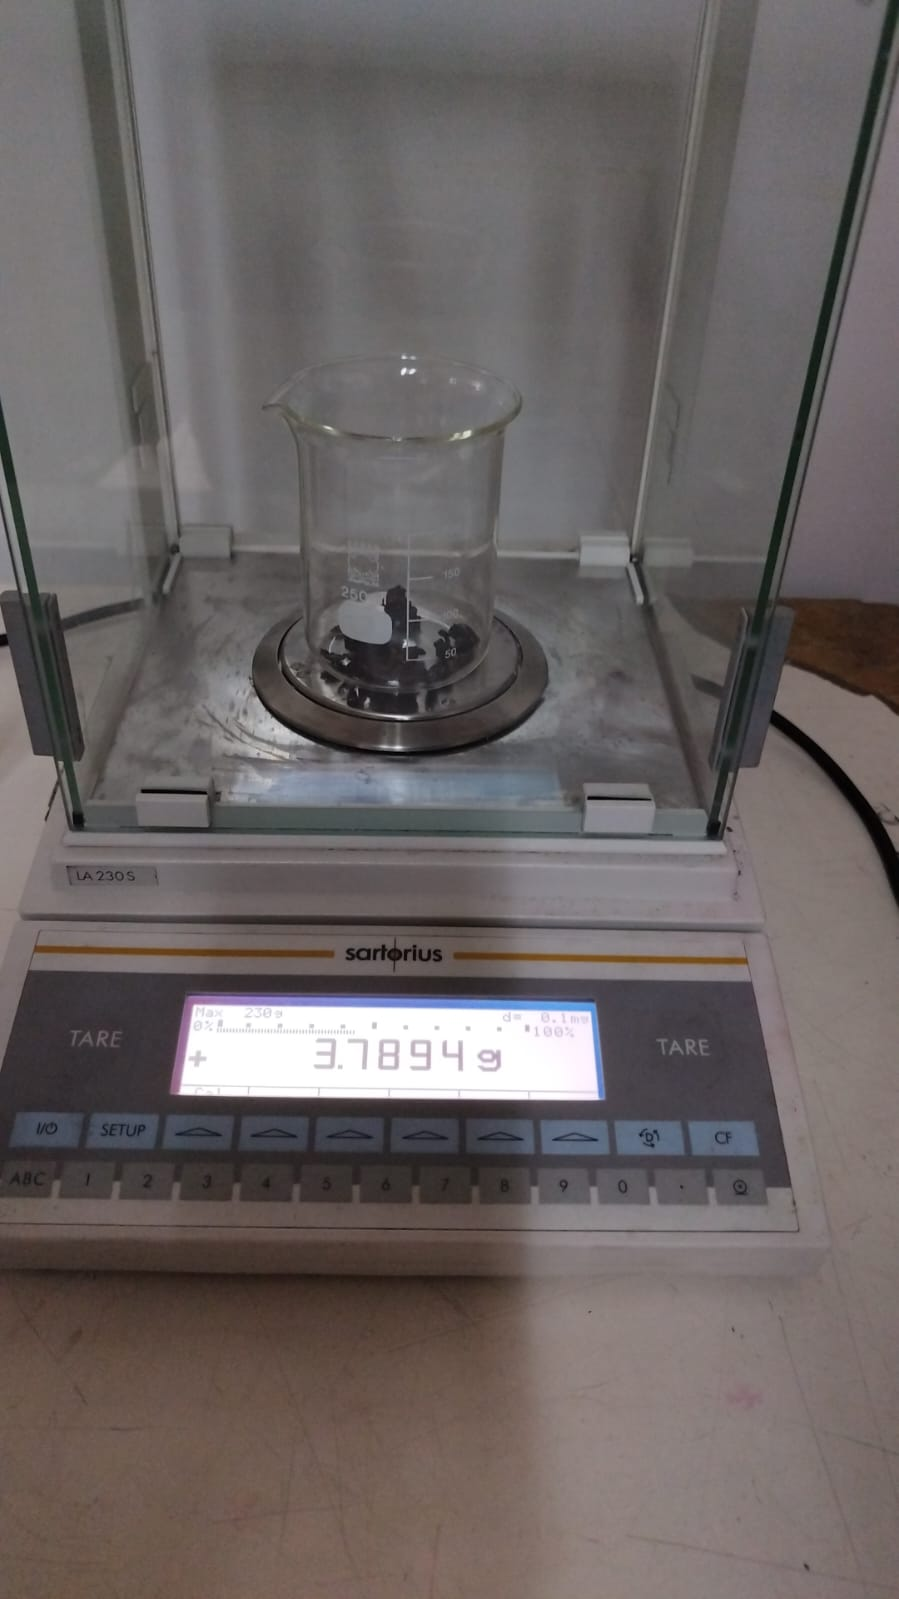
\includegraphics[width=\textwidth]{images/Pruebas/Resultados/muestra_2.jpeg}
        \caption{Pesaje}
        \label{fg:m2_pesaje}
    \end{subfigure}
    \hfill
    \begin{subfigure}[b]{0.32\textwidth}
        \centering
        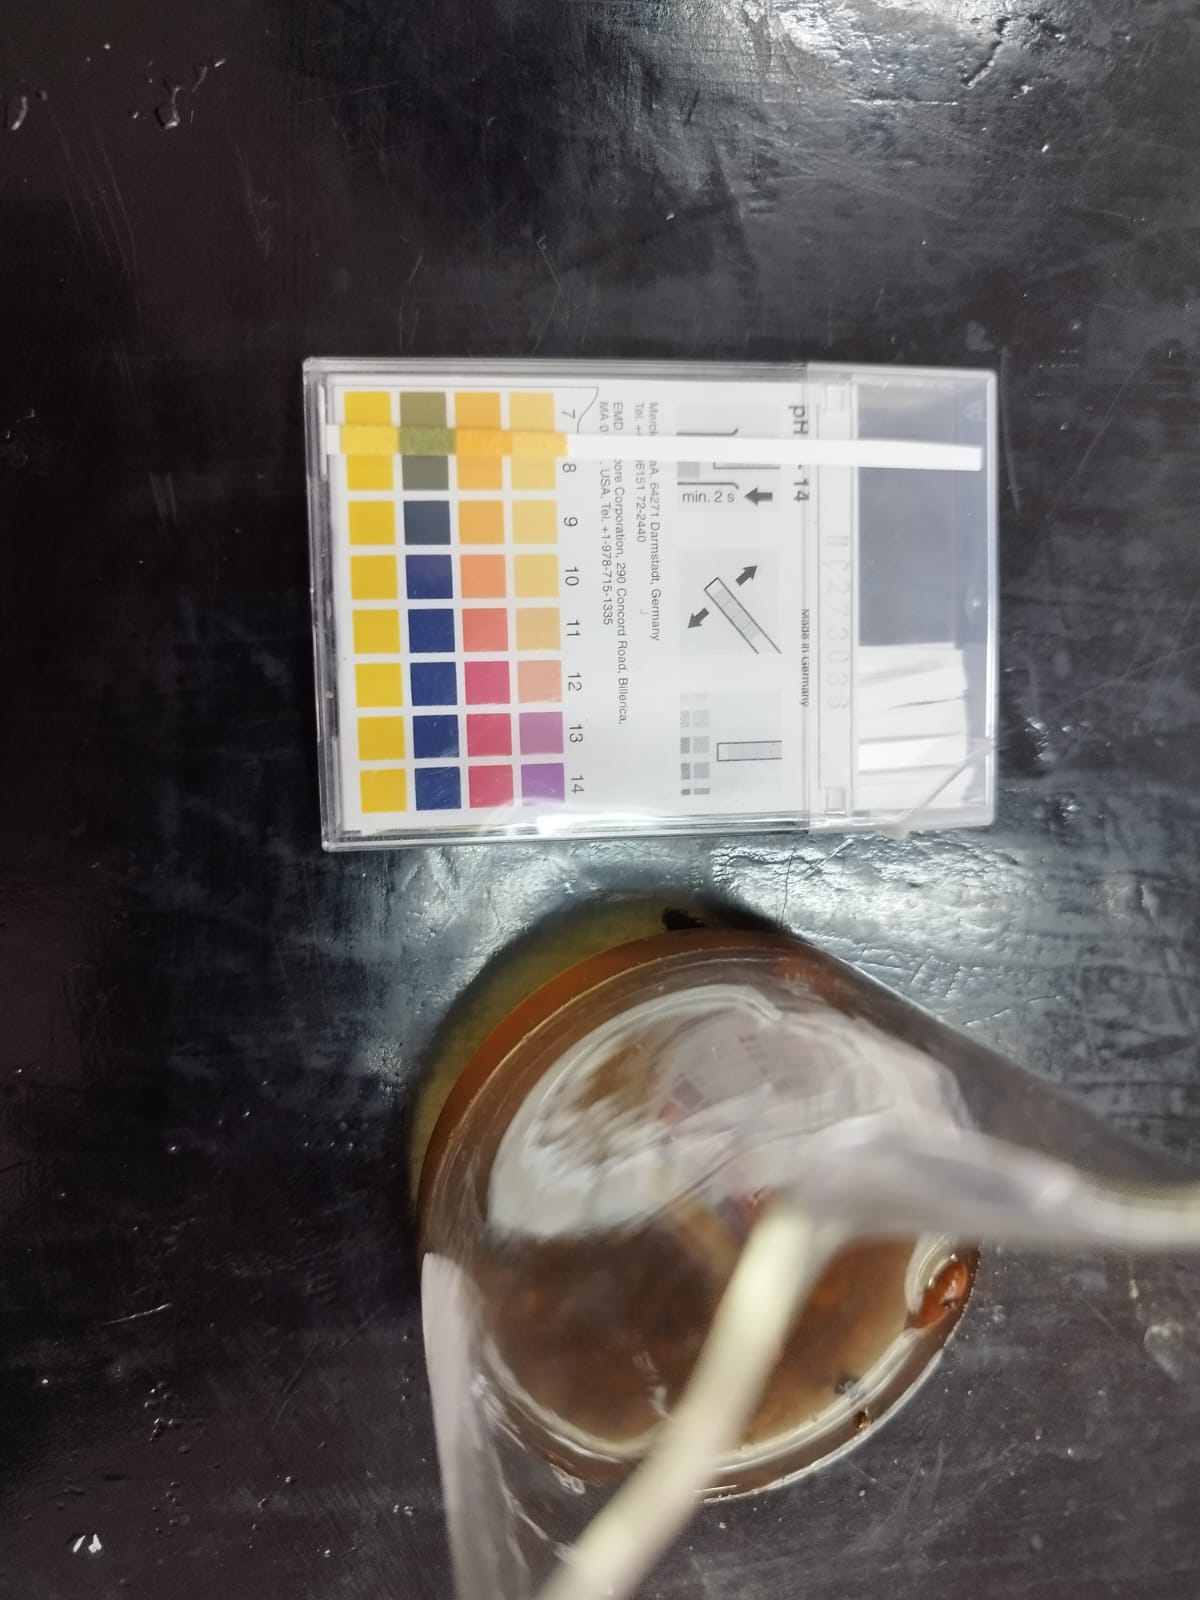
\includegraphics[width=\textwidth]{images/Pruebas/Resultados/muestra_2_colorimetria.jpeg}
        \caption{Comparativa colorimétrica}
        \label{fg:m2_color}
    \end{subfigure}
    \hfill
    \begin{subfigure}[b]{0.32\textwidth}
        \centering
        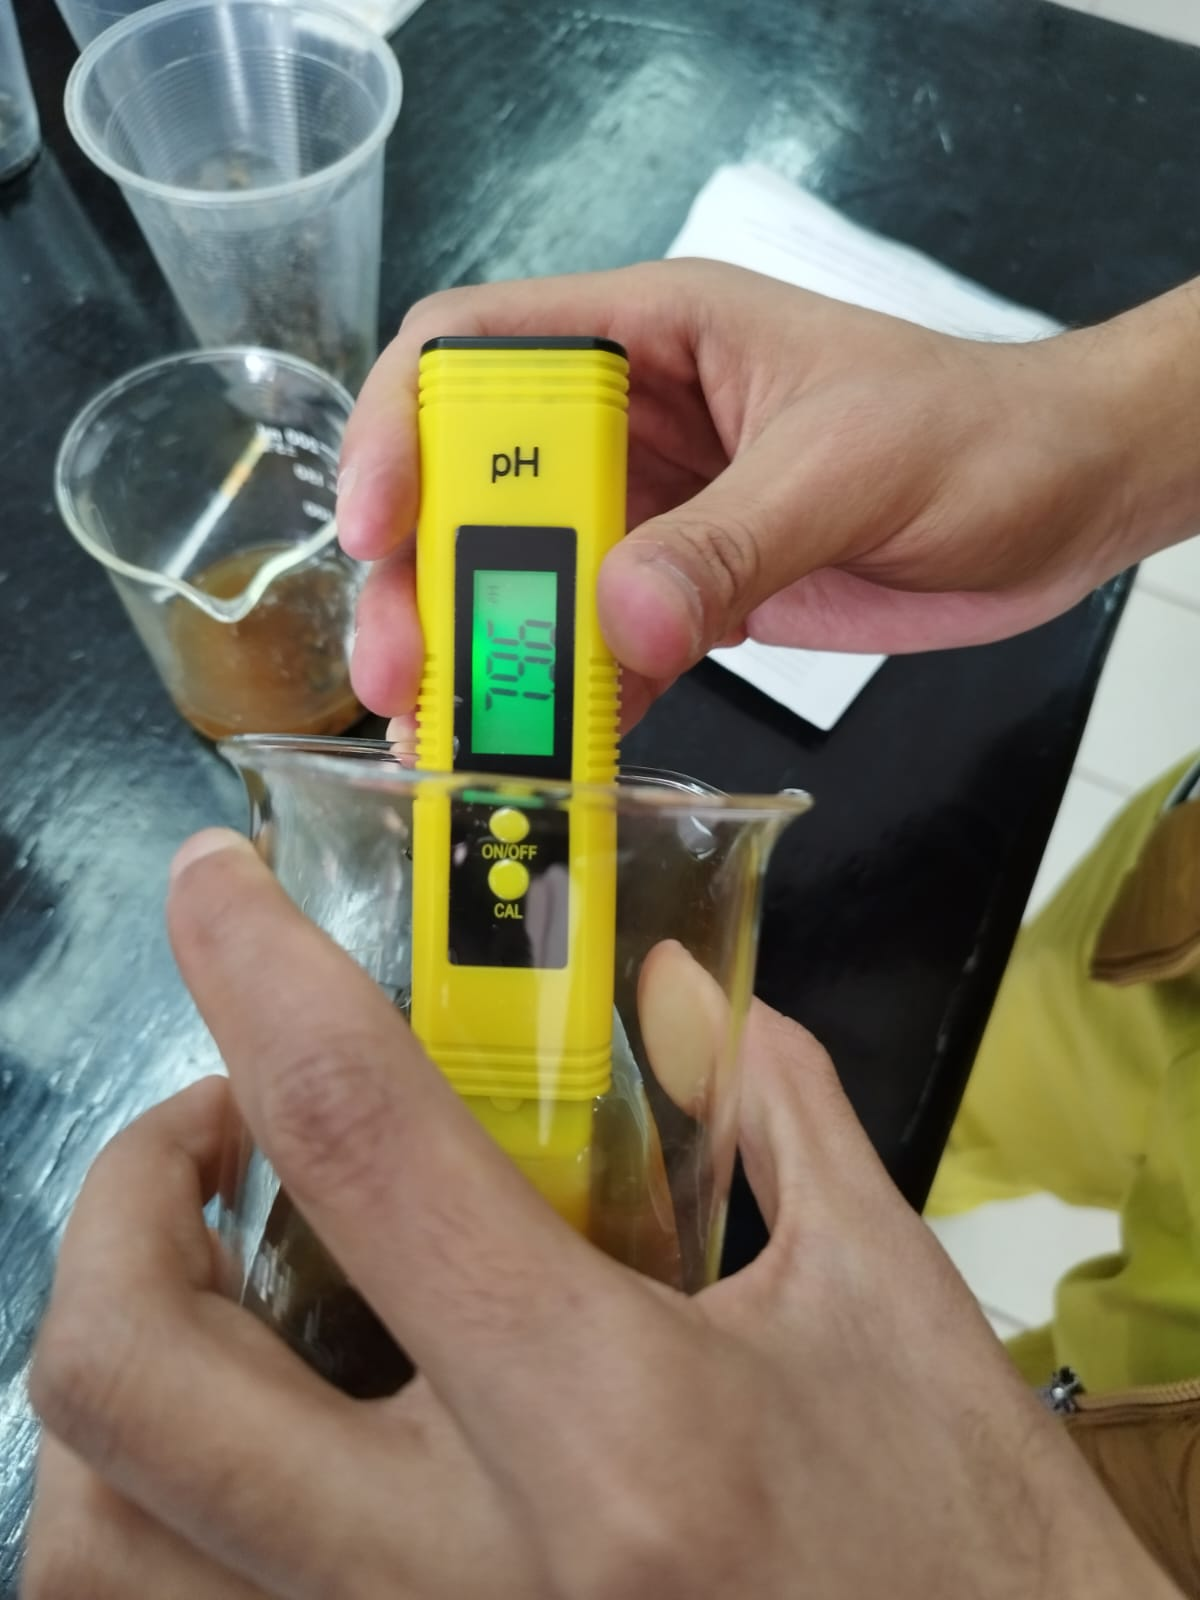
\includegraphics[width=\textwidth]{images/Pruebas/Resultados/muestra_2_phmetro.jpeg}
        \caption{Lectura de pHmetro}
        \label{fg:m2_ph}
    \end{subfigure}
    \caption{Proceso de medición de pH — Muestra 2}
    \label{fg:muestra2_proceso}
\end{figure}

Las imágenes de la Figura \ref{fg:muestra2_proceso} evidencian una consistencia aún muy húmeda y una coloración similar a la de la muestra 1. 

En contraste, la tercera muestra (prueba 3) presentó las mejores condiciones de procesamiento: los residuos fueron totalmente triturados hasta partículas de aproximadamente 3 mm, lo que favoreció un compost de aspecto similar a la tierra, con partícula fina, color café oscuro, olor a durazno y humedad mínima. Esta muestra se deshacía al soltarla y alcanzó un pH de 7.62, el más cercano a la neutralidad entre las pruebas exitosas.

\begin{figure}[H]
    \centering
    \begin{subfigure}[b]{0.30\textwidth}
        \centering
        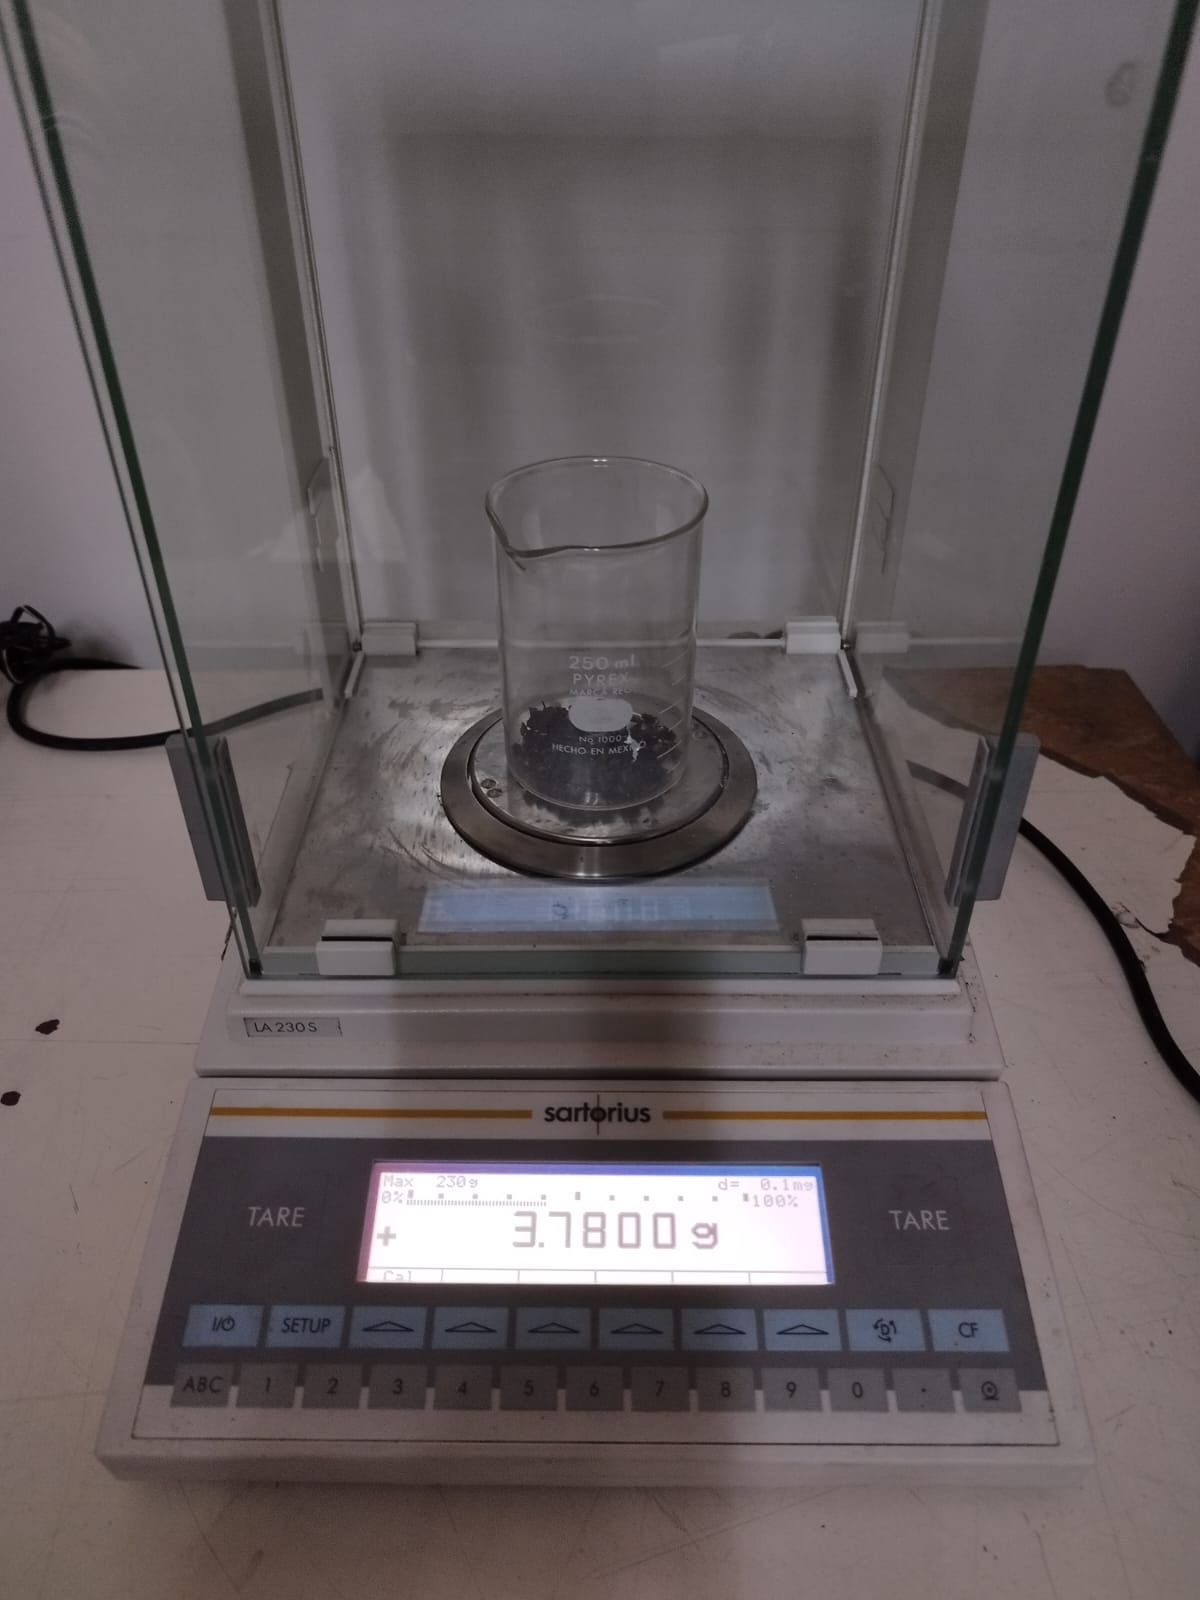
\includegraphics[width=\textwidth]{images/Pruebas/Resultados/muestra_3.jpeg}
        \caption{Pesaje}
        \label{fg:m3_pesaje}
    \end{subfigure}
    \hfill
    \begin{subfigure}[b]{0.32\textwidth}
        \centering
        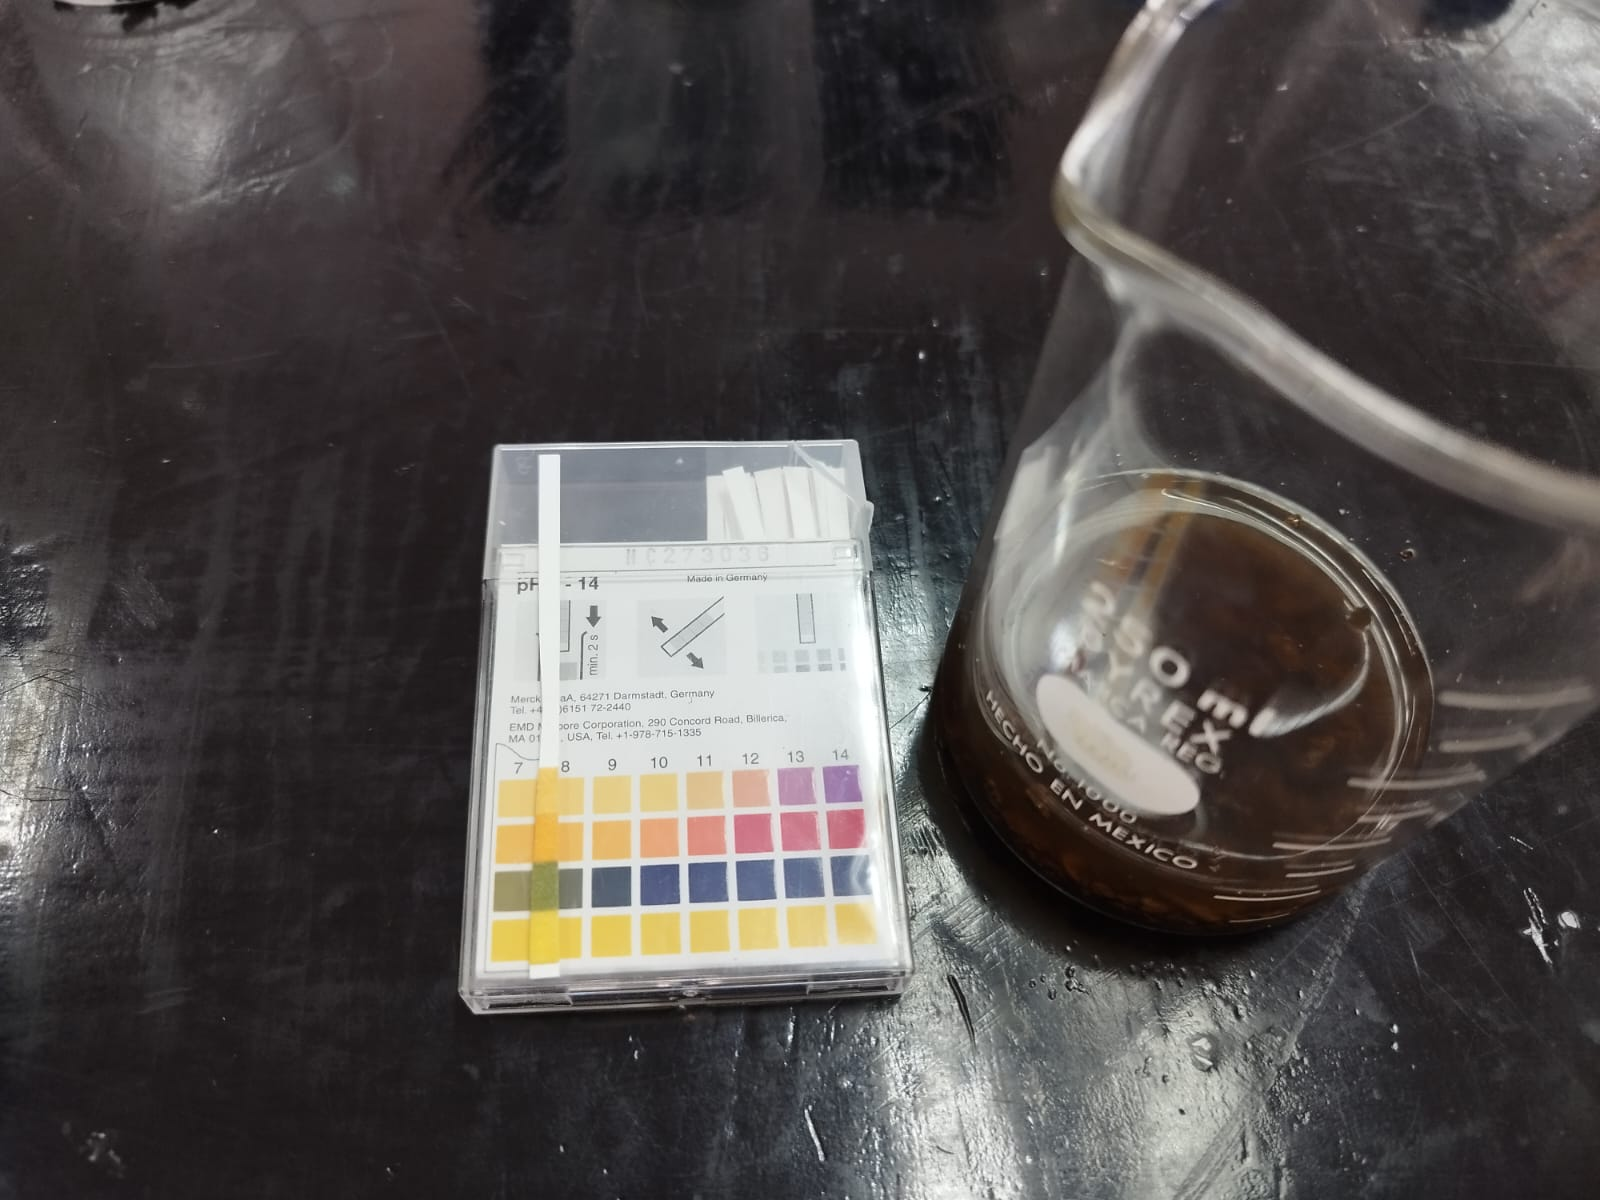
\includegraphics[width=\textwidth]{images/Pruebas/Resultados/muestra_3_colorimetria.jpeg}
        \caption{Comparativa colorimétrica}
        \label{fg:m3_color}
    \end{subfigure}
    \hfill
    \begin{subfigure}[b]{0.30\textwidth}
        \centering
        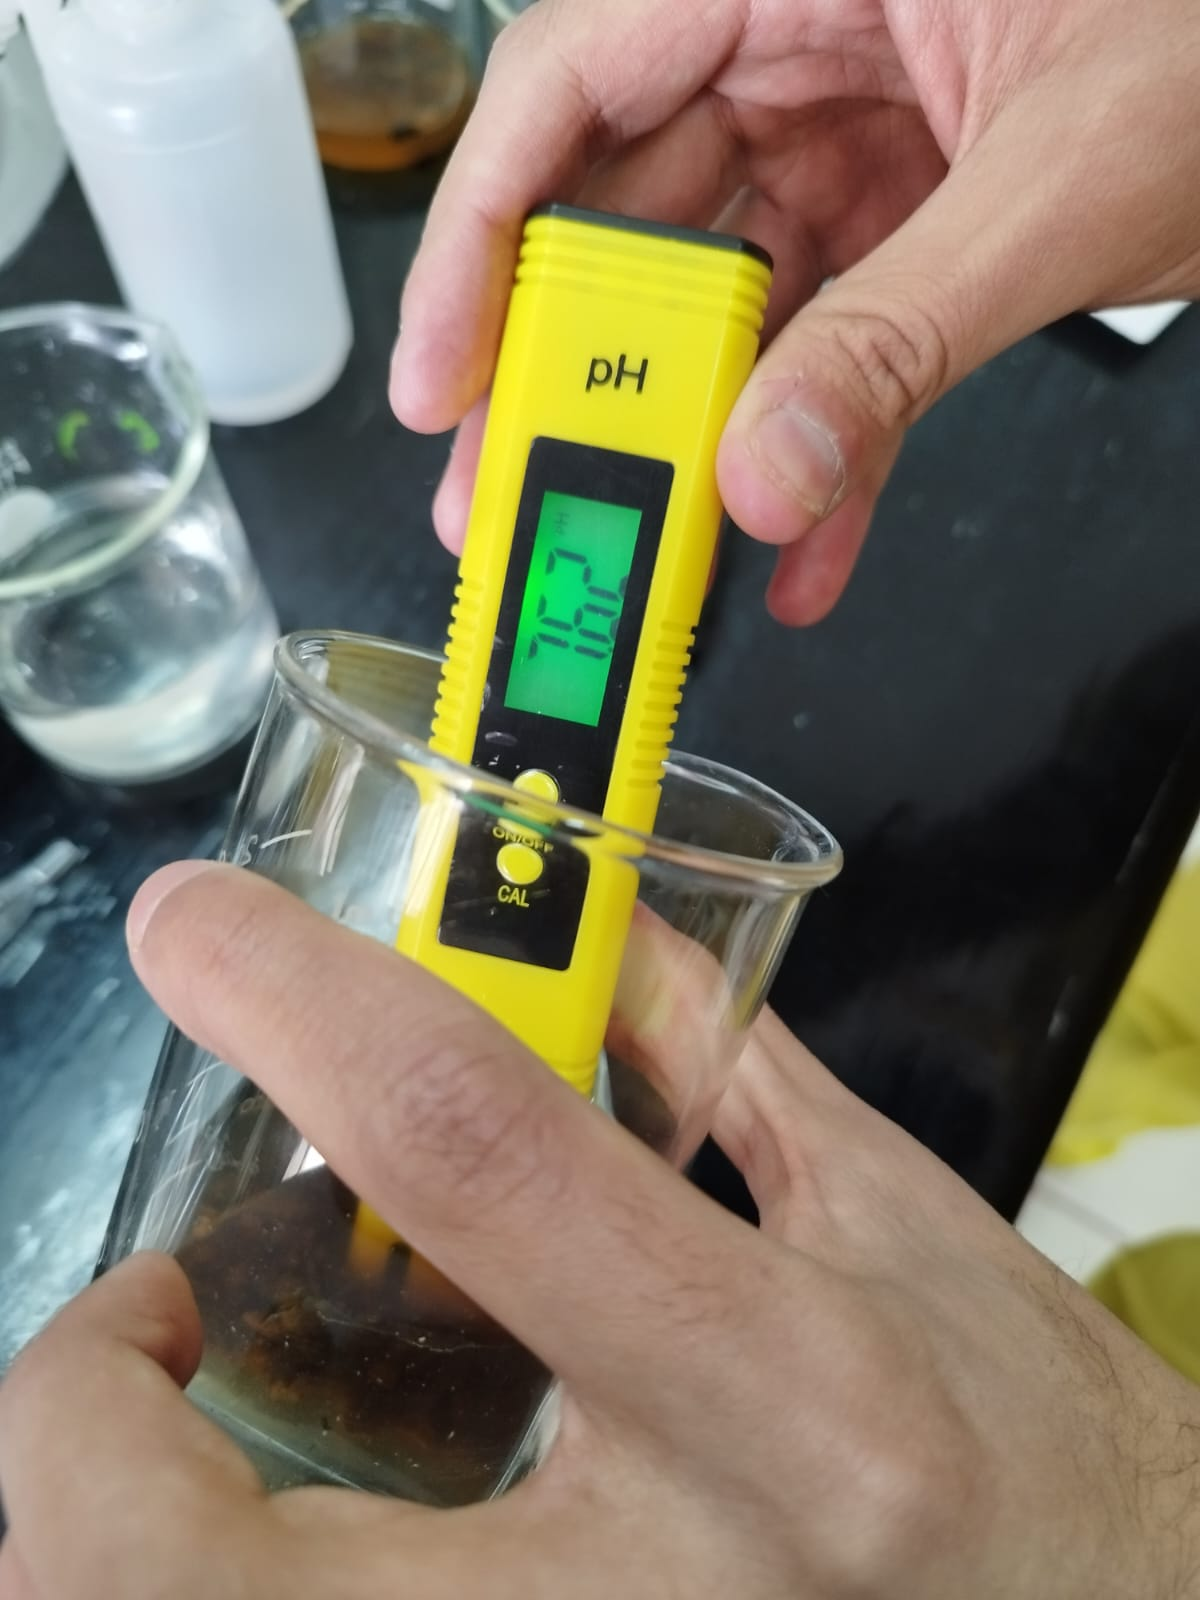
\includegraphics[width=\textwidth]{images/Pruebas/Resultados/muestra_3_phmetro.jpeg}
        \caption{Lectura de pHmetro}
        \label{fg:m3_ph}
    \end{subfigure}
    \caption{Proceso de medición de pH — Muestra 3}
    \label{fg:muestra3_proceso}
\end{figure}

La Figura \ref{fg:muestra3_proceso} documenta estas características visuales.

La cuarta muestra (prueba 4) correspondió a una preparación mixta: la mitad de los residuos fue triturada y la otra mitad picada. El compost resultante fue homogéneo, con humedad moderada y un olor frutal agradable, alcanzando un pH de 5.33.

\begin{figure}[H]
    \centering
    \begin{subfigure}[b]{0.32\textwidth}
        \centering
        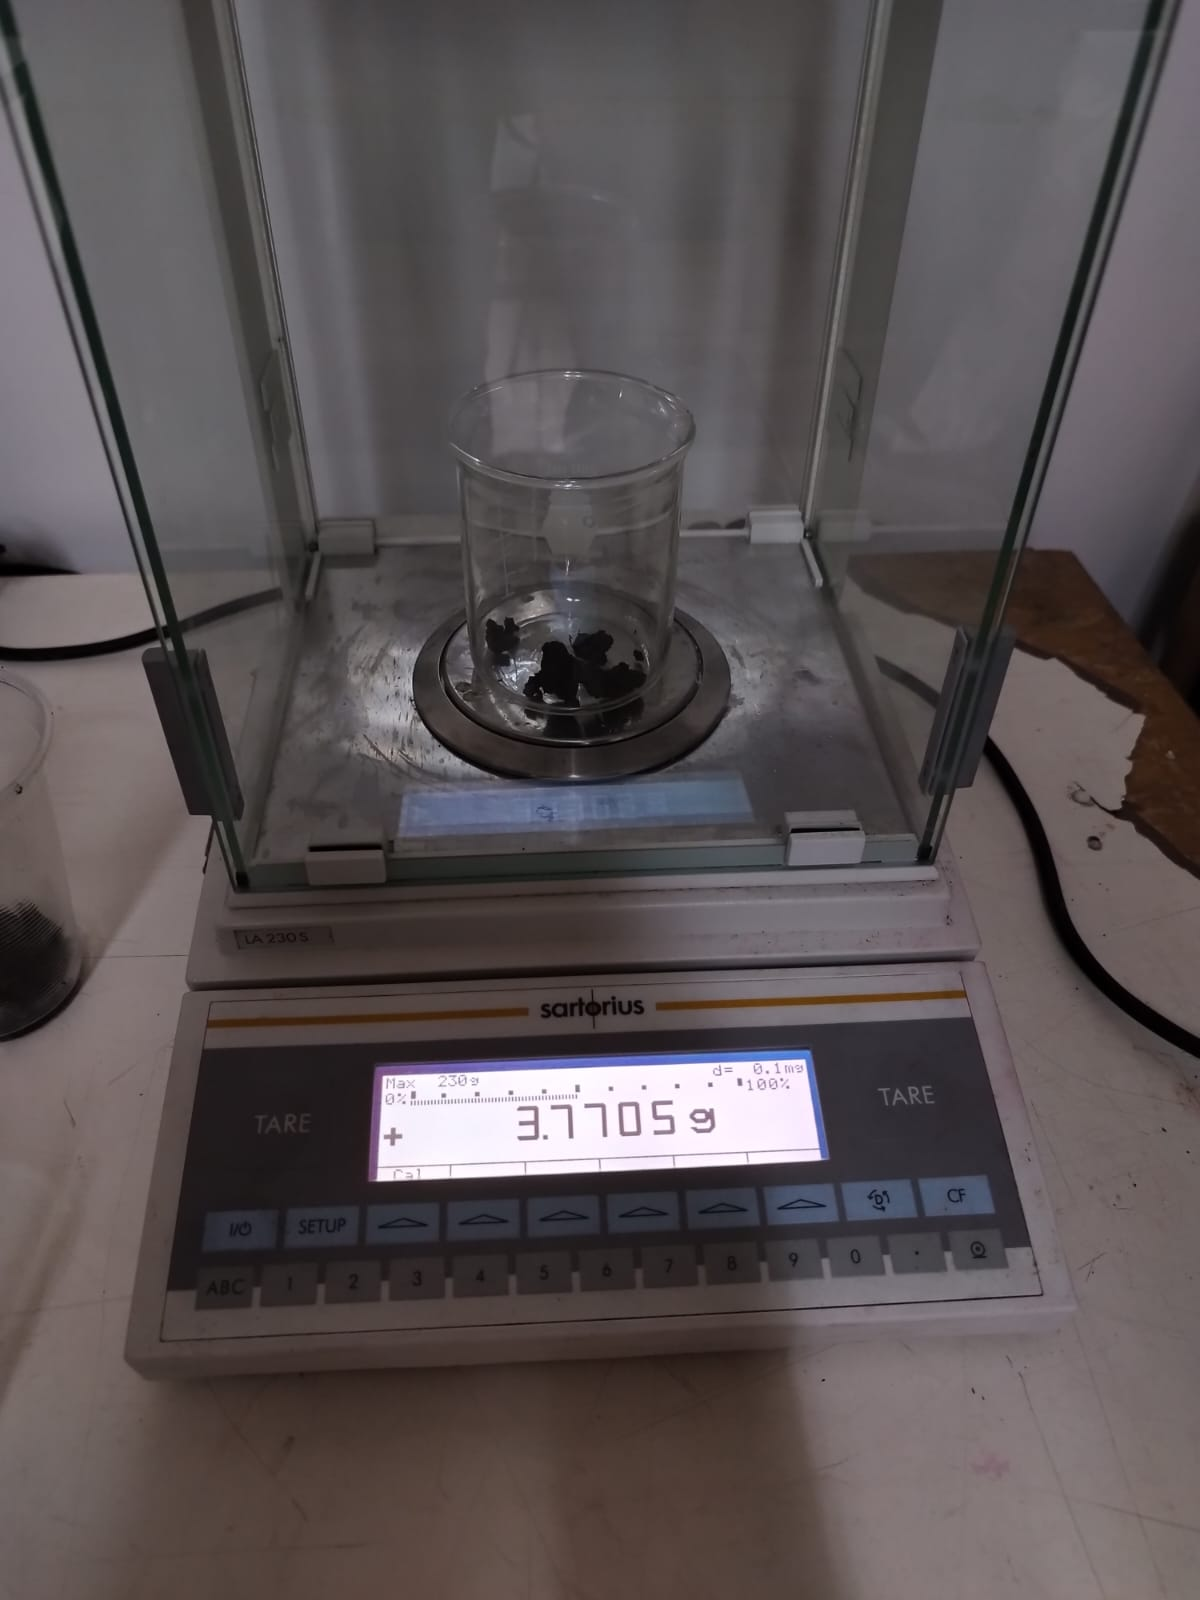
\includegraphics[width=\textwidth]{images/Pruebas/Resultados/muestra_4.jpeg}
        \caption{Pesaje}
        \label{fg:m4_pesaje}
    \end{subfigure}
    \hfill
    \begin{subfigure}[b]{0.32\textwidth}
        \centering
        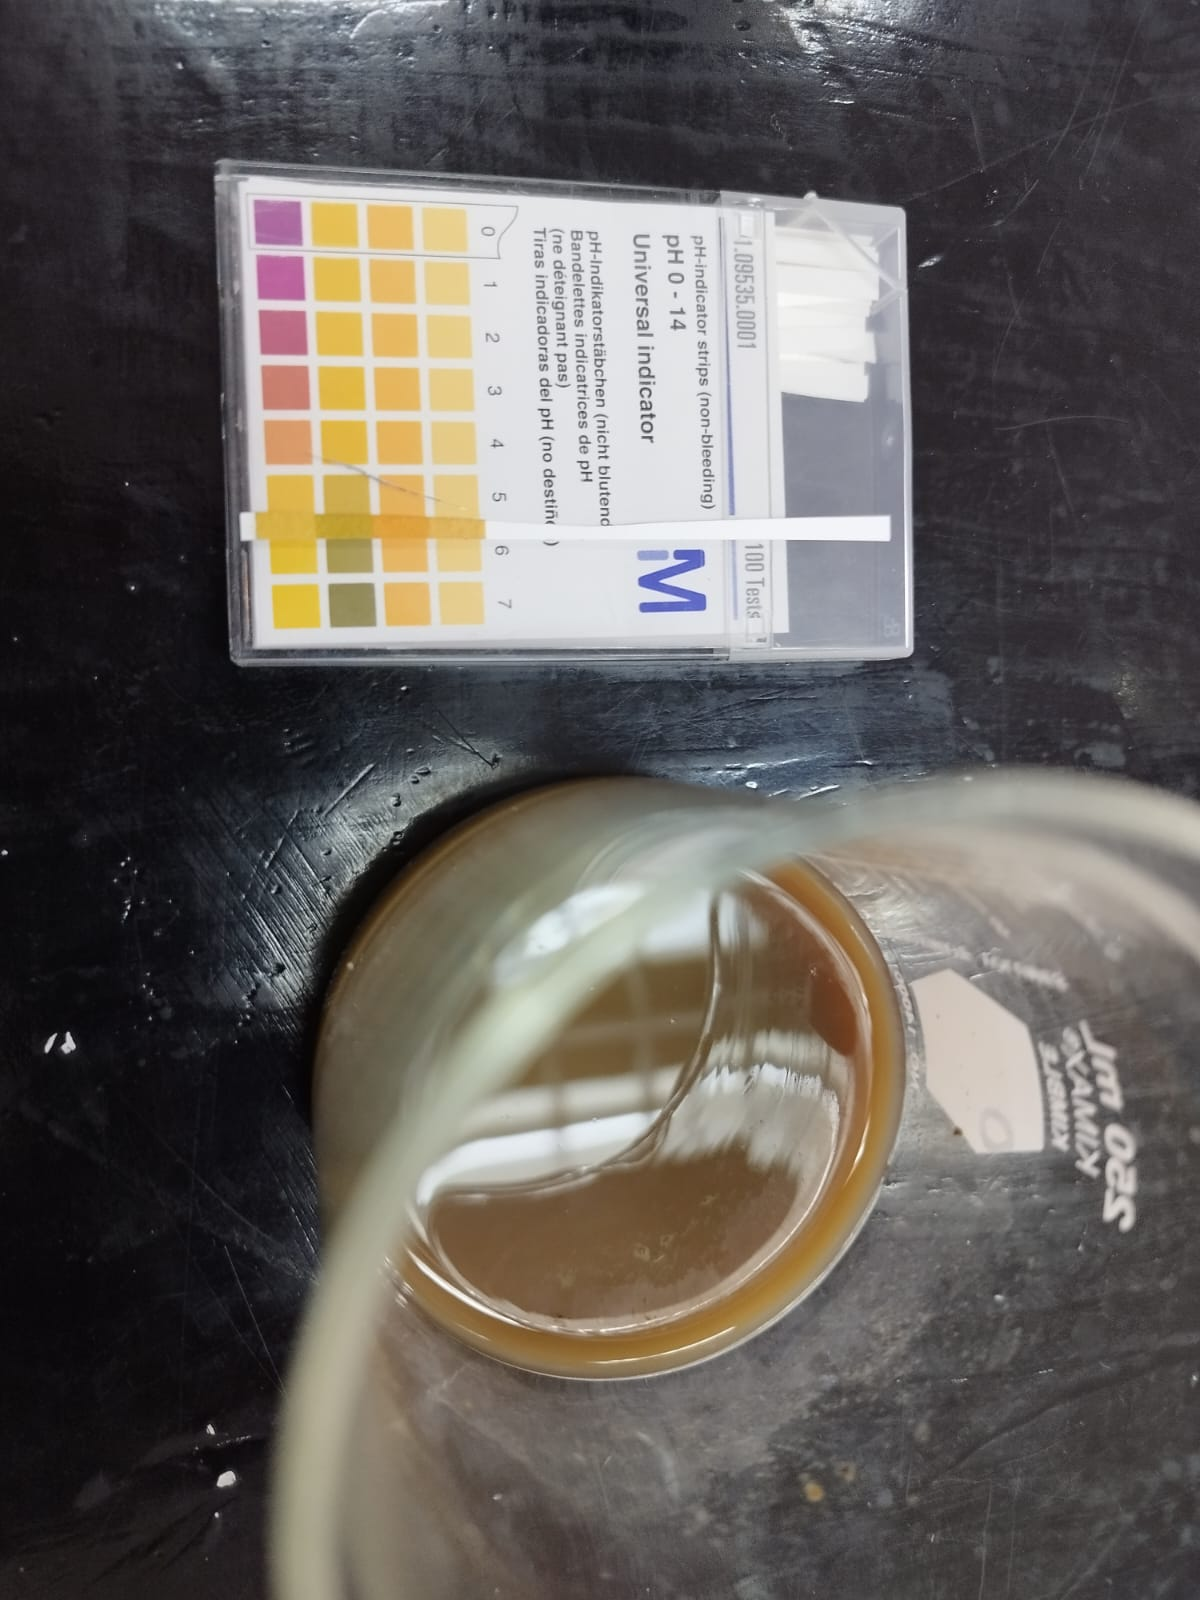
\includegraphics[width=\textwidth]{images/Pruebas/Resultados/muestra_4_colorimetria.jpeg}
        \caption{Comparativa colorimétrica}
        \label{fg:m4_color}
    \end{subfigure}
    \hfill
    \begin{subfigure}[b]{0.32\textwidth}
        \centering
        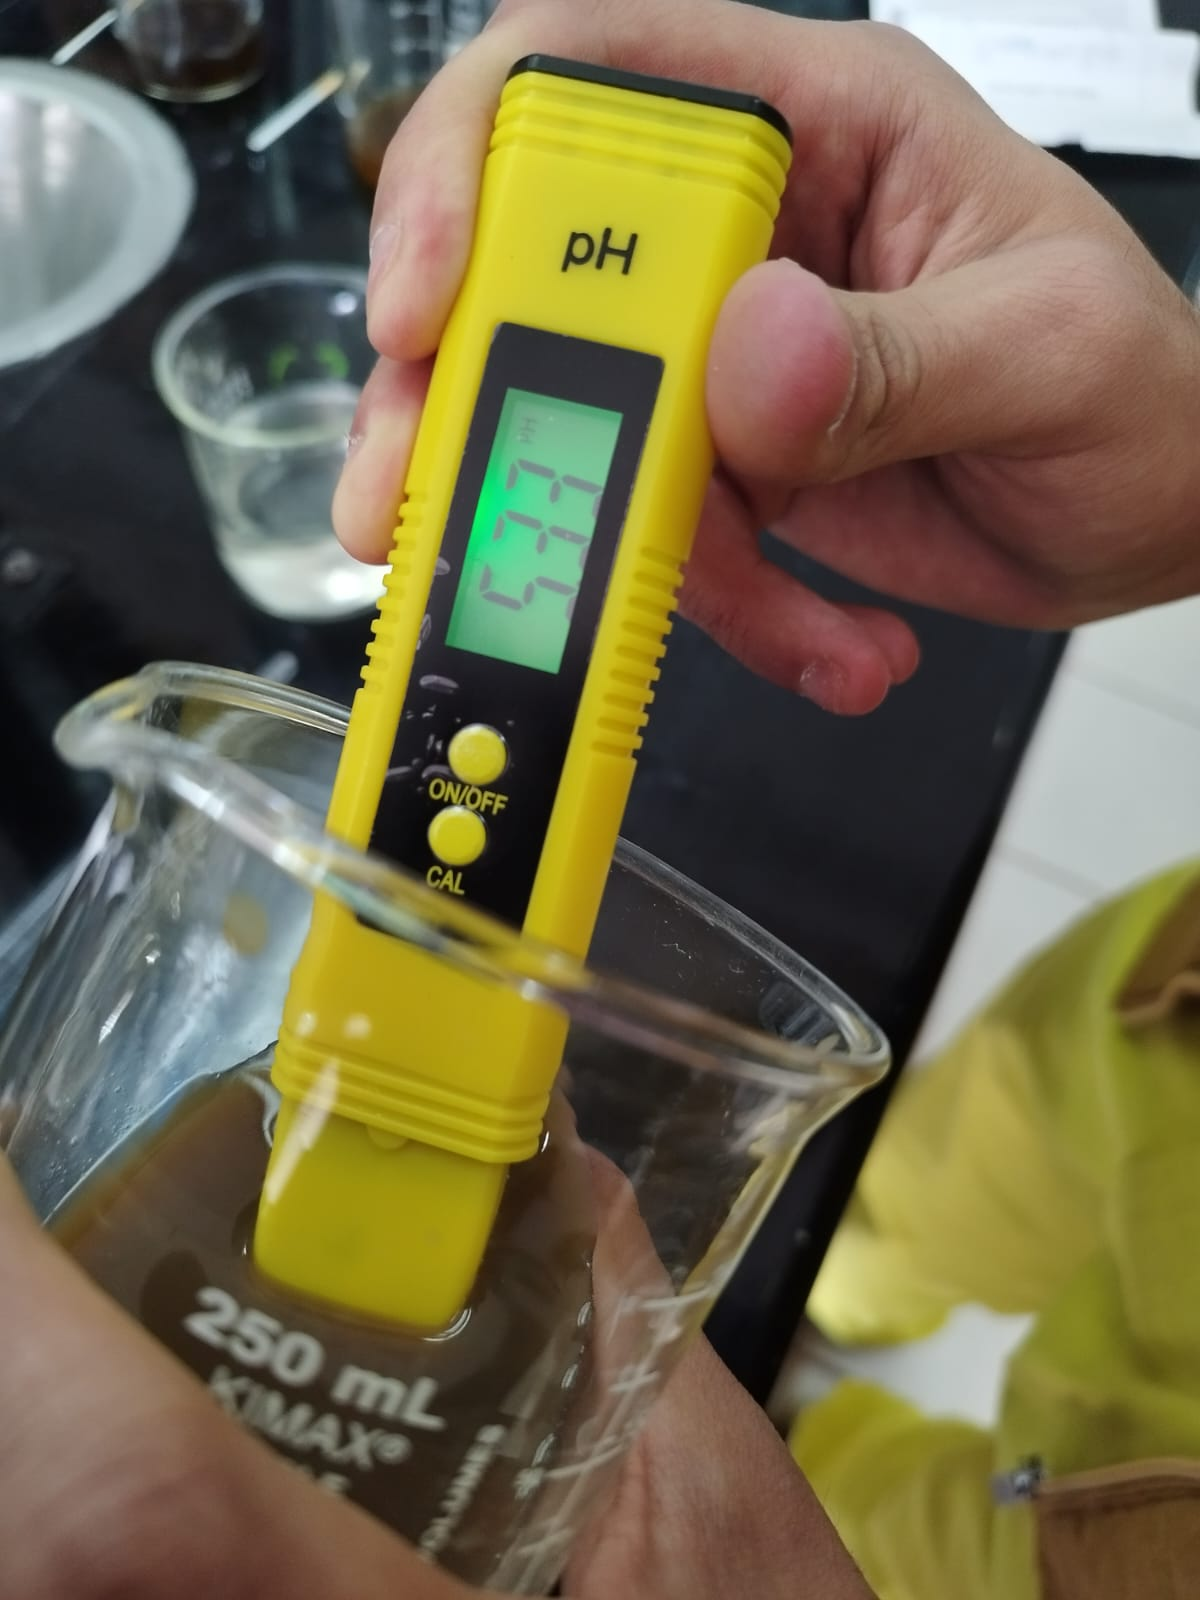
\includegraphics[width=\textwidth]{images/Pruebas/Resultados/muestra_4_phmetro.jpeg}
        \caption{Lectura de pHmetro}
        \label{fg:m4_ph}
    \end{subfigure}
    \caption{Proceso de medición de pH — Muestra 4}
    \label{fg:muestra4_proceso}
\end{figure}

La Figura \ref{fg:muestra4_proceso} muestra el pesaje, la comparativa colorimétrica y la lectura de pH para esta muestra. 

Finalmente, la quinta muestra (prueba 5) se obtuvo a partir de residuos frescos y muy húmedos que solo fueron picados. El compost presentó una consistencia pastosa, descrita como similar a mole o lodo, con color café oscuro y olor agradable, pero con un exceso de agua evidente. Su pH final fue de 7.15, y el rendimiento alcanzó el 48.4\,\%, el más alto entre las pruebas exitosas.

\begin{figure}[H]
    \centering
    \begin{subfigure}[b]{0.32\textwidth}
        \centering
        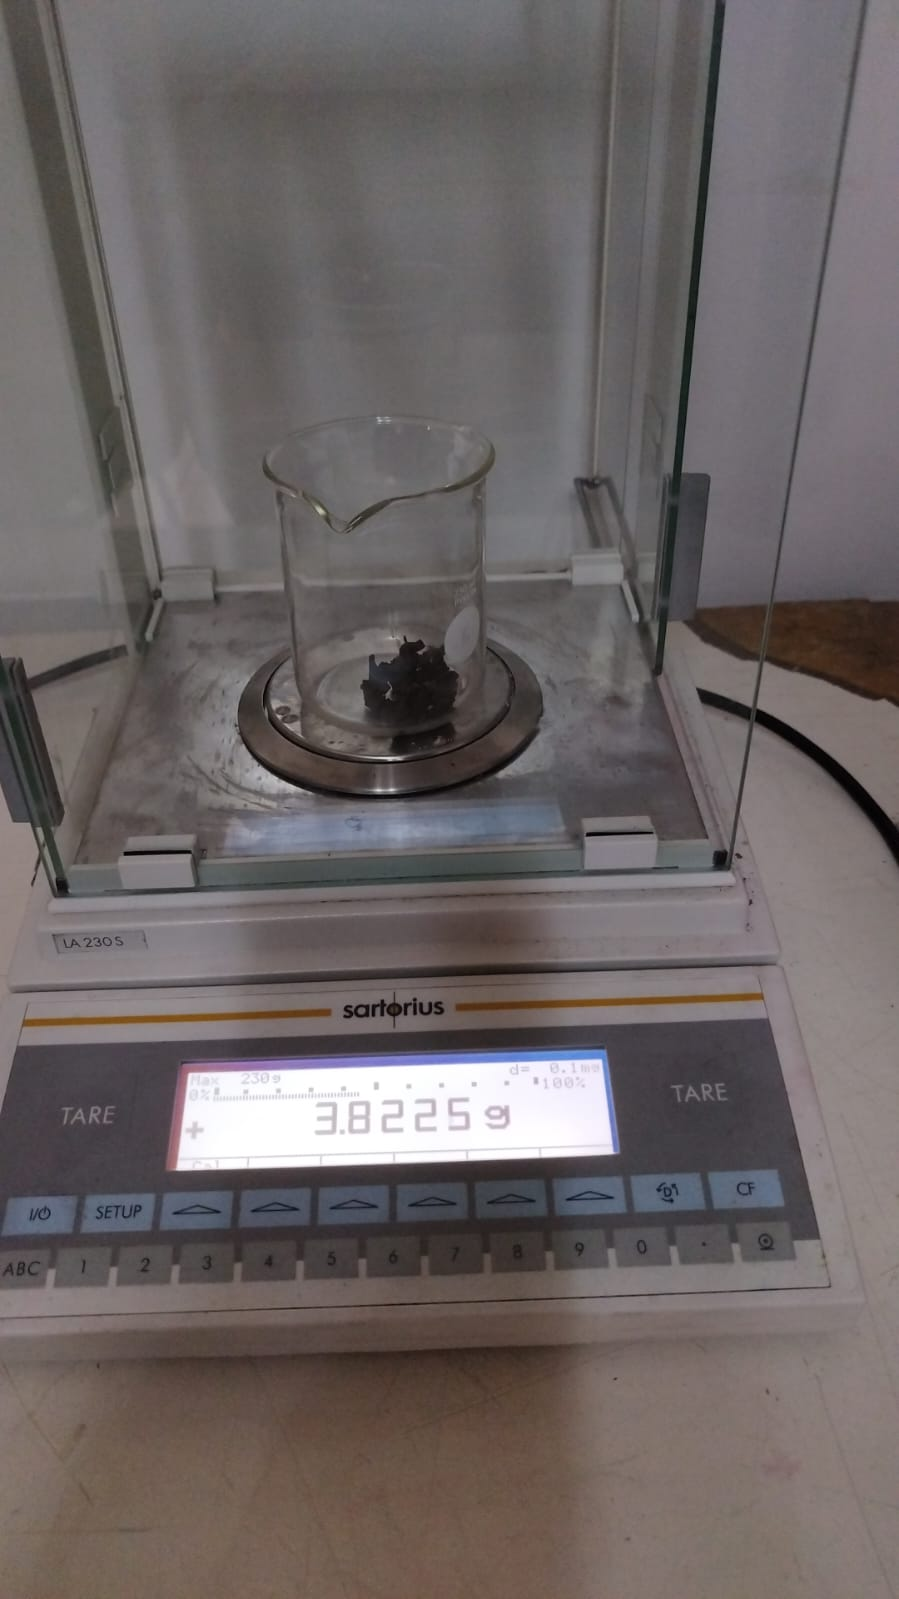
\includegraphics[width=\textwidth]{images/Pruebas/Resultados/muestra_5.jpeg}
        \caption{Pesaje}
        \label{fg:m5_pesaje}
    \end{subfigure}
    \hfill
    \begin{subfigure}[b]{0.32\textwidth}
        \centering
        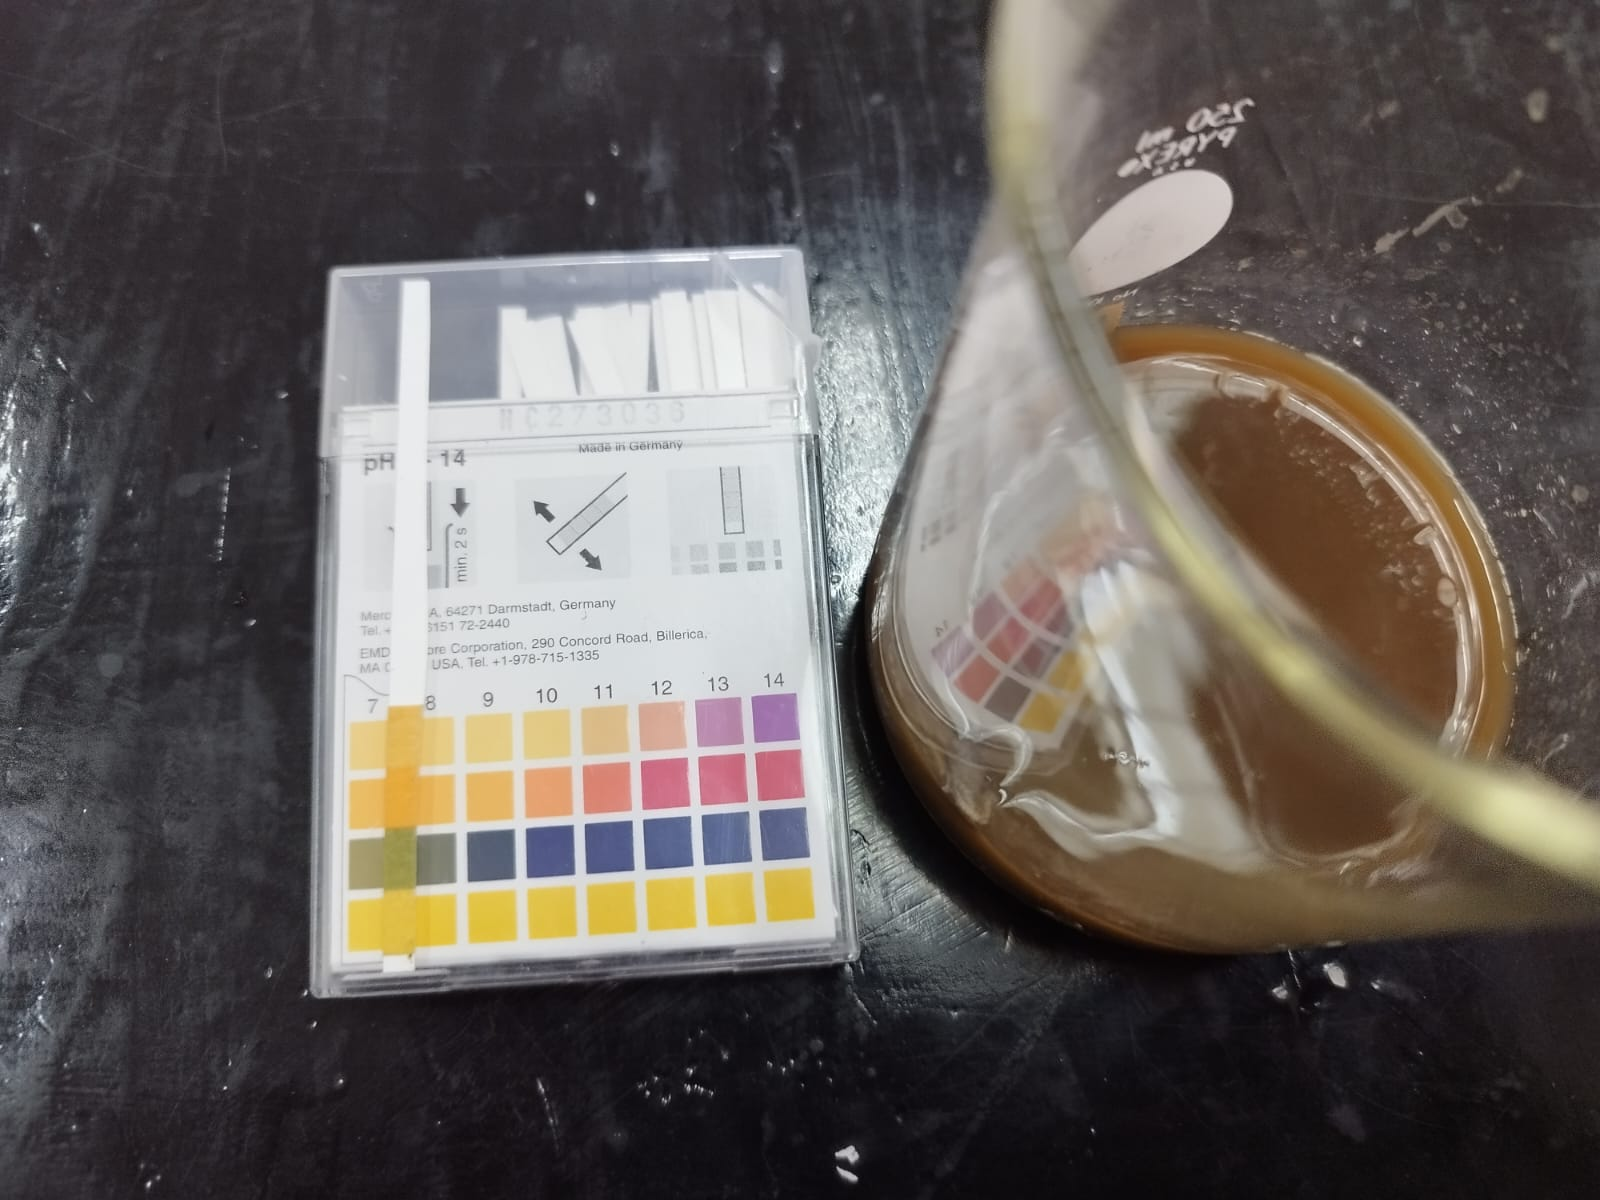
\includegraphics[width=\textwidth]{images/Pruebas/Resultados/muestra_5_colorimetria.jpeg}
        \caption{Comparativa colorimétrica}
        \label{fg:m5_color}
    \end{subfigure}
    \hfill
    \begin{subfigure}[b]{0.32\textwidth}
        \centering
        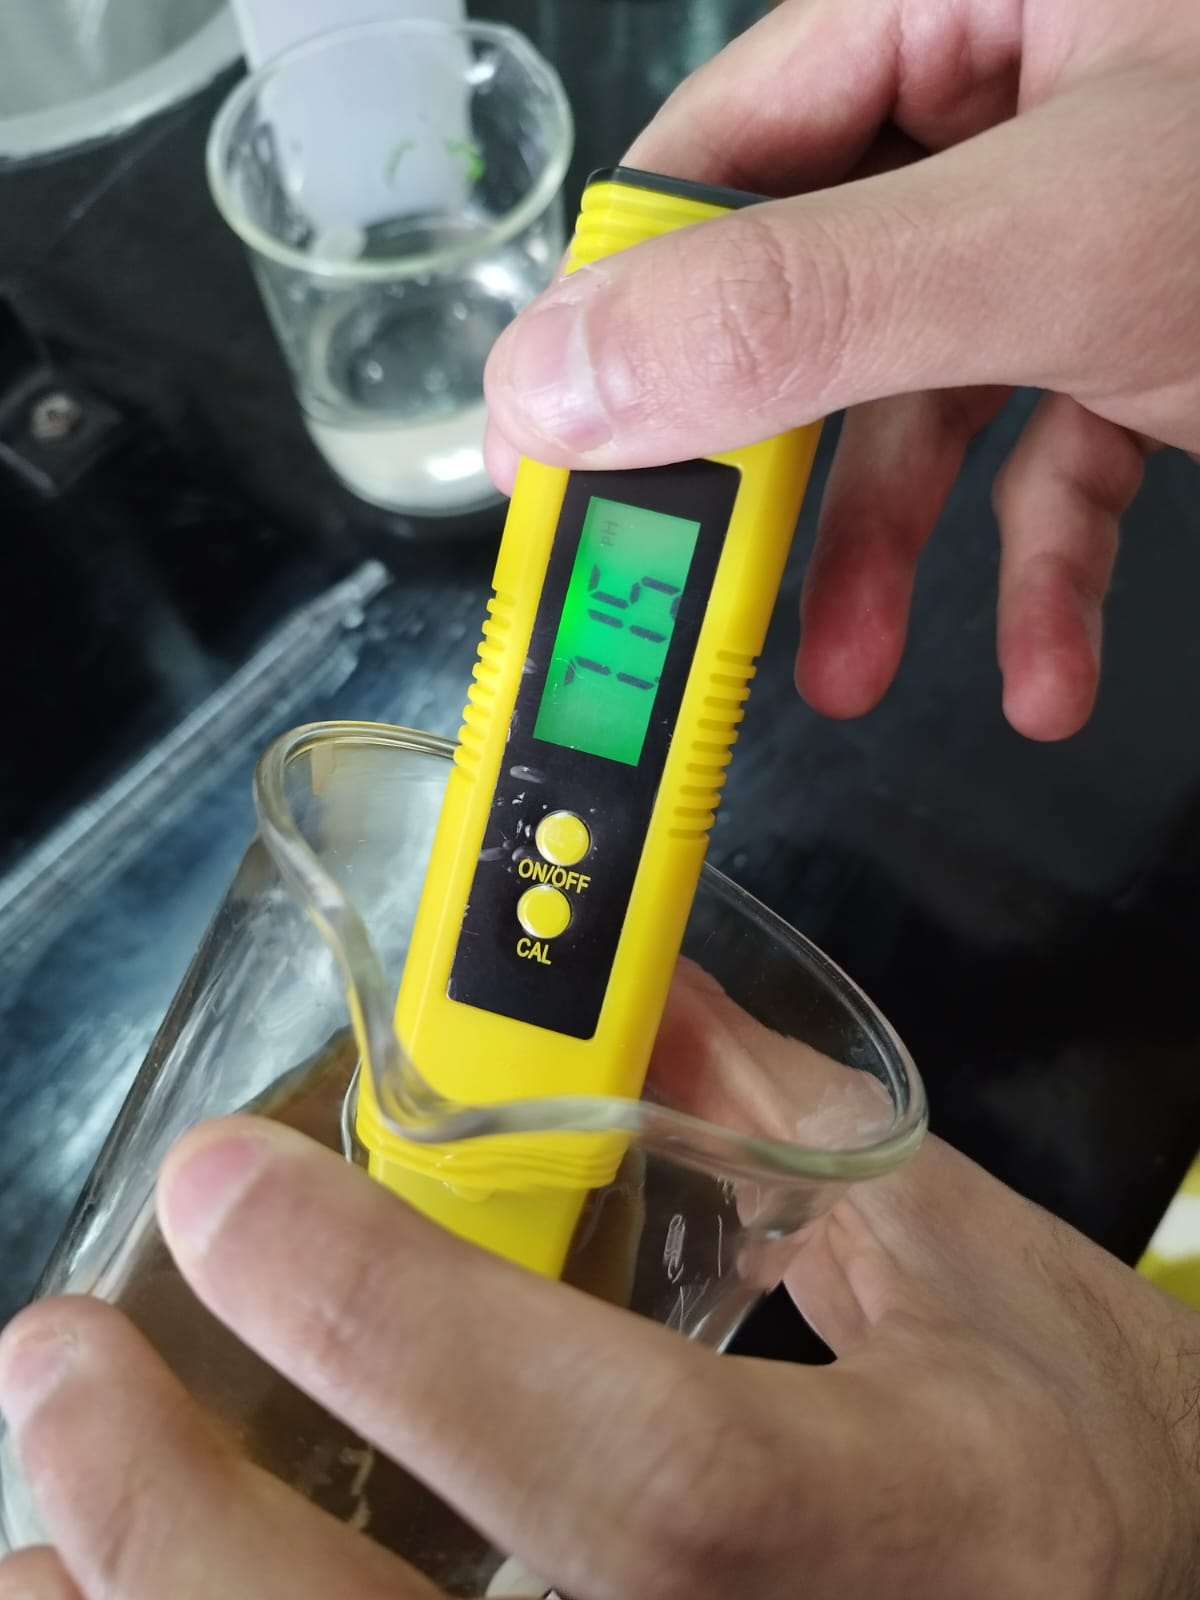
\includegraphics[width=\textwidth]{images/Pruebas/Resultados/muestra_5_phmetro.jpeg}
        \caption{Lectura de pHmetro}
        \label{fg:m5_ph}
    \end{subfigure}
    \caption{Proceso de medición de pH — Muestra 5}
    \label{fg:muestra5_proceso}
\end{figure}